%% abtex2-modelo-trabalho-academico.tex, v-1.9.7 laurocesar
%% Copyright 2012-2018 by abnTeX2 group at http://www.abntex.net.br/ 
%%
%% This work may be distributed and/or modified under the
%% conditions of the LaTeX Project Public License, either version 1.3
%% of this license or (at your option) any later version.
%% The latest version of this license is in
%%   http://www.latex-project.org/lppl.txt
%% and version 1.3 or later is part of all distributions of LaTeX
%% version 2005/12/01 or later.
%%
%% This work has the LPPL maintenance status `maintained'.
%% 
%% The Current Maintainer of this work is the abnTeX2 team, led
%% by Lauro César Araujo. Further information are available on 
%% http://www.abntex.net.br/
%%
%% This work consists of the files abntex2-modelo-trabalho-academico.tex,
%% abntex2-modelo-include-comandos and abntex2-modelo-references.bib
%%

% ------------------------------------------------------------------------
% ------------------------------------------------------------------------
% abnTeX2: Modelo de Trabalho Academico (tese de doutorado, dissertacao de
% mestrado e trabalhos monograficos em geral) em conformidade com 
% ABNT NBR 14724:2011: Informacao e documentacao - Trabalhos academicos -
% Apresentacao
% ------------------------------------------------------------------------
% ------------------------------------------------------------------------

\documentclass[
	% -- opções da classe memoir --
	12pt,				% tamanho da fonte
	openright,			% capítulos começam em pág ímpar (insere página vazia caso preciso)
	oneside,			% para impressão em recto e verso use 'twoside'. Oposto a 'oneside'
	a4paper,			% tamanho do papel. 
	% -- opções da classe abntex2 --
	%chapter=TITLE,		% títulos de capítulos convertidos em letras maiúsculas
	%section=TITLE,		% títulos de seções convertidos em letras maiúsculas
	%subsection=TITLE,	% títulos de subseções convertidos em letras maiúsculas
	%subsubsection=TITLE,% títulos de subsubseções convertidos em letras maiúsculas
	% -- opções do pacote babel --
	english,			% idioma adicional para hifenização
	brazil				% o último idioma é o principal do documento
	]{abntex2}

% ---
% Pacotes básicos 
% ---
\usepackage{lmodern}			% Usa a fonte Latin Modern			
\usepackage[T1]{fontenc}		% Selecao de codigos de fonte.
\usepackage[utf8]{inputenc}		% Codificacao do documento (conversão automática dos acentos)
\usepackage{indentfirst}		% Indenta o primeiro parágrafo de cada seção.
\usepackage{color}				% Controle das cores
\usepackage{graphicx}			% Inclusão de gráficos
\usepackage{microtype} 			% para melhorias de justificação
\usepackage{amsmath}
\usepackage{mathtools}
% ---
		
% ---
% Pacotes adicionais, usados apenas no âmbito do Modelo Canônico do abnteX2
% ---
\usepackage{lipsum}				% para geração de dummy text
% ---

% ---
% Pacotes de citações
% ---
\usepackage[brazilian,hyperpageref]{backref}	 % Paginas com as citações na bibl
\usepackage[alf, abnt-etal-list=0]{abntex2cite}	% Citações padrão ABNT
\citebrackets()

% --- 
% CONFIGURAÇÕES DE PACOTES
% --- 

% ---
% Configurações do pacote backref
% Usado sem a opção hyperpageref de backref
\renewcommand{\backrefpagesname}{Citado na(s) página(s):~}
% Texto padrão antes do número das páginas
\renewcommand{\backref}{}
% Define os textos da citação
\renewcommand*{\backrefalt}[4]{
	\ifcase #1 %
		Nenhuma citação no texto.%
	\or
		Citado na página #2.%
	\else
		Citado #1 vezes nas páginas #2.%
	\fi}%
% ---

% ---
% Informações de dados para CAPA e FOLHA DE ROSTO
% ---
\titulo{Modelagem de Superfícies Reconfiguráveis Inteligentes com Camada Única e Contínua usando Método dos Momentos}
\autor{André Vinícius de Souza Lages}
\local{Belém}
\data{2024}
\orientador{Karlo Queiroz da Costa}
\coorientador{João Crisóstomo Weyl Albuquerque Costa}
\instituicao{Universidade Federal do Pará}
\instituicaounidade{Instituto de Tecnologia}
\instituicaosubunidade{Programa de Pós-Graduação em Engenharia Elétrica - PPGEE}


\tipotrabalho{Tese (Doutorado)}
% O preambulo deve conter o tipo do trabalho, o objetivo, 
% o nome da instituição e a área de concentração 
\preambulo{Qualificação de Tese de Doutorado apresentado no Programa de Pós-graduação em Engenharia Elétrica do Instituto de Tecnologia como requisito parcial para obtenção do grau de doutor.}
% ---


% ---
% Configurações de aparência do PDF final

% alterando o aspecto da cor azul
\definecolor{blue}{RGB}{41,5,195}

% informações do PDF
\makeatletter
\hypersetup{
     	%pagebackref=true,
		pdftitle={\@title}, 
		pdfauthor={\@author},
    	pdfsubject={\imprimirpreambulo},
	    pdfcreator={LaTeX with abnTeX2},
		pdfkeywords={abnt}{latex}{abntex}{abntex2}{trabalho acadêmico}, 
		colorlinks=true,       		% false: boxed links; true: colored links
    	linkcolor=black,          	% color of internal links
    	citecolor=black,        		% color of links to bibliography
    	filecolor=black,      		% color of file links
		urlcolor=black,
		bookmarksdepth=4
}
\makeatother
% --- 

% ---
% Posiciona figuras e tabelas no topo da página quando adicionadas sozinhas
% em um página em branco. Ver https://github.com/abntex/abntex2/issues/170
\makeatletter
\setlength{\@fptop}{5pt} % Set distance from top of page to first float
\makeatother
% ---

% ---
% Possibilita criação de Quadros e Lista de quadros.
% Ver https://github.com/abntex/abntex2/issues/176
%
\newcommand{\quadroname}{Quadro}
\newcommand{\listofquadrosname}{Lista de quadros}

\newfloat[chapter]{quadro}{loq}{\quadroname}
\newlistof{listofquadros}{loq}{\listofquadrosname}
\newlistentry{quadro}{loq}{0}

% configurações para atender às regras da ABNT
\setfloatadjustment{quadro}{\centering}
\counterwithout{quadro}{chapter}
\renewcommand{\cftquadroname}{\quadroname\space} 
\renewcommand*{\cftquadroaftersnum}{.\hfill}

\setfloatlocations{quadro}{hbtp} % Ver https://github.com/abntex/abntex2/issues/176
% ---

% --- 
% Espaçamentos entre linhas e parágrafos 
% --- 

% O tamanho do parágrafo é dado por:
\setlength{\parindent}{1.3cm}

% Controle do espaçamento entre um parágrafo e outro:
\setlength{\parskip}{0.2cm}  % tente também \onelineskip

% ---
% compila o indice
% ---
\makeindex
% ---

% ----
% Início do documento
% ----
\begin{document}

% Seleciona o idioma do documento (conforme pacotes do babel)
%\selectlanguage{english}
\selectlanguage{brazil}

% Retira espaço extra obsoleto entre as frases.
\frenchspacing 

% ----------------------------------------------------------
% ELEMENTOS PRÉ-TEXTUAIS
% ----------------------------------------------------------
% \pretextual

% ---
% Capa
% ---
\imprimircapa
% ---

% ---
% Folha de rosto
% (o * indica que haverá a ficha bibliográfica)
% ---
\imprimirfolhaderosto*
% ---

% ---
% Inserir a ficha bibliografica
% ---

% Isto é um exemplo de Ficha Catalográfica, ou ``Dados internacionais de
% catalogação-na-publicação''. Você pode utilizar este modelo como referência. 
% Porém, provavelmente a biblioteca da sua universidade lhe fornecerá um PDF
% com a ficha catalográfica definitiva após a defesa do trabalho. Quando estiver
% com o documento, salve-o como PDF no diretório do seu projeto e substitua todo
% o conteúdo de implementação deste arquivo pelo comando abaixo:
%
% \begin{fichacatalografica}
%     \includepdf{fig_ficha_catalografica.pdf}
% \end{fichacatalografica}

\begin{fichacatalografica}
	\sffamily
	\vspace*{\fill}					% Posição vertical
	\begin{center}					% Minipage Centralizado
	\fbox{\begin{minipage}[c][8cm]{13.5cm}		% Largura
	\small
	Solicite sua ficha catalográfica em: \url{http://bcficat.ufpa.br/}
	\end{minipage}}
	\end{center}
\end{fichacatalografica}
% ---

% ---
% Inserir errata
% ---
%\begin{errata}
%Elemento opcional da %\cite{NBR14724:2011}. Exemplo:

%\vspace{\onelineskip}

%FERRIGNO, C. R. A. \textbf{Tratamento de neoplasias ósseas apendiculares com
%reimplantação de enxerto ósseo autólogo autoclavado associado ao plasma
%rico em plaquetas}: estudo crítico na cirurgia de preservação de membro em
%cães. 2011. 128 f. Tese (Livre-Docência) - Faculdade de Medicina Veterinária e
%Zootecnia, Universidade de São Paulo, São Paulo, 2011.

%\begin{table}[htb]
%\center
%\footnotesize
%\begin{tabular}{|p{1.4cm}|p{1cm}|p{3cm}|p{3cm}|}
%  \hline
%   \textbf{Folha} & \textbf{Linha}  & \textbf{Onde se lê}  & \textbf{Leia-se}  \\
%    \hline
%    1 & 10 & auto-conclavo & autoconclavo\\
%   \hline
%\end{tabular}
%\end{table}

%\end{errata}
% ---

% ---
% Inserir folha de aprovação
% ---

% Isto é um exemplo de Folha de aprovação, elemento obrigatório da NBR
% 14724/2011 (seção 4.2.1.3). Você pode utilizar este modelo até a aprovação
% do trabalho. Após isso, substitua todo o conteúdo deste arquivo por uma
% imagem da página assinada pela banca com o comando abaixo:
%
% \begin{folhadeaprovacao}
% \includepdf{folhadeaprovacao_final.pdf}
% \end{folhadeaprovacao}
%
\begin{folhadeaprovacao}

  \begin{center}
    {\ABNTEXchapterfont\large\imprimirautor}

    \vspace*{\fill}\vspace*{\fill}
    \begin{center}
      \ABNTEXchapterfont\bfseries\Large\imprimirtitulo
    \end{center}
    \vspace*{\fill}
    
    \hspace{.45\textwidth}
    \begin{minipage}{.5\textwidth}
        \imprimirpreambulo
    \end{minipage}%
    \vspace*{\fill}
   \end{center}
        
   Conceito: \rule{3cm}{.1pt}
   
   \imprimirlocal, 30 de janeiro de 2025.
   
   \vspace{1cm}
   \begin{center}
   BANCA EXAMINADORA
   \end{center}
    


   \assinatura{\textbf{\imprimirorientador} - Orientador \\ UFPA}
   \assinatura{\textbf{\imprimircoorientador} - Coorientador \\ UFPA}
   \assinatura{\textbf{André Mendes Cavalcante   }\\Ericsson}
   \assinatura{\textbf{Gilvan Soares Borges} \\ IFPA}
      

  
\end{folhadeaprovacao}
% ---

% ---
% Dedicatória
% ---
\begin{dedicatoria}
   \vspace*{\fill}
   \centering
   \noindent
   \textit{ Escreva sua dedicatória aqui.} \vspace*{\fill}
\end{dedicatoria}
% ---

% ---
% Agradecimentos
% ---
\begin{agradecimentos}
Os agradecimentos principais são a Deus por me dar forças e iluminar muitas pessoas, pais e mães do céu que tem me ajudado nesse caminho torutoso depois de muitas adversidades na minha vida. Em especial, aos professores Karlo e João, ao André da Ericsson, por me acolherem, me darem uma oportunidade, serem compreensivos com meus problemas pessoais, me deixarem acrediar que sou capaz de me superar com amor, dedicação...  

\end{agradecimentos}
% ---

% ---
% Epígrafe
% ---
\begin{epigrafe}
    \vspace*{\fill}
	\begin{flushright}
		\textit{``Escreva sua epígrafe aqui''\\
		(Fulano de Tal, 19XX)}
	\end{flushright}
\end{epigrafe}
% ---

% ---
% RESUMOS
% ---

% resumo em português
\setlength{\absparsep}{18pt} % ajusta o espaçamento dos parágrafos do resumo
\begin{resumo}
 Segundo a \cite{NBR6028:2003}, o resumo deve ressaltar o
 objetivo, o método, os resultados e as conclusões do documento. A ordem e a extensão
 destes itens dependem do tipo de resumo (informativo ou indicativo) e do
 tratamento que cada item recebe no documento original. O resumo deve ser
 precedido da referência do documento, com exceção do resumo inserido no
 próprio documento. (\ldots) As palavras-chave devem figurar logo abaixo do
 resumo, antecedidas da expressão Palavras-chave:, separadas entre si por
 ponto e finalizadas também por ponto.

 \textbf{Palavras-chave}: latex. abntex. editoração de texto.
\end{resumo}

% resumo em inglês
\begin{resumo}[Abstract]
 \begin{otherlanguage*}{english}
   This is the english abstract.

   \vspace{\onelineskip}
 
   \noindent 
   \textbf{Keywords}: latex. abntex. text editoration.
 \end{otherlanguage*}
\end{resumo}

% ---

% ---
% inserir lista de ilustrações
% ---
\pdfbookmark[0]{\listfigurename}{lof}
\listoffigures*
\cleardoublepage
% ---

% ---
% inserir lista de quadros
% ---
\pdfbookmark[0]{\listofquadrosname}{loq}
\listofquadros*
\cleardoublepage
% ---

% ---
% inserir lista de tabelas
% ---
\pdfbookmark[0]{\listtablename}{lot}
\listoftables*
\cleardoublepage
% ---

% ---
% inserir lista de abreviaturas e siglas
% ---
\begin{siglas}
  \item[5G] Quinta Geração de Tecnologia Móvel
  \item[6G] Sexta Geração de Tecnologia Móvel
  
\end{siglas}
% ---

% ---
% inserir lista de símbolos
% ---
\begin{simbolos}
  \item[$ \overline{E}_i $] Vetor Campo Elétrico incidente
  \item[$ \overline{E}_s $] Vetor Campo Elétrico de Espalhamento
  \item[$ \epsilon $] Permissividade do meio
  \item[$ \mu $] Permeabilidade do meio
  \item[$ \overline{J} $] Vetor densidade de corrente elétrica
  
\end{simbolos}
% ---

% ---
% inserir o sumario
% ---
\pdfbookmark[0]{\contentsname}{toc}
\tableofcontents*
\cleardoublepage
% ---



% ----------------------------------------------------------
% ELEMENTOS TEXTUAIS
% ----------------------------------------------------------
\textual

% ----------------------------------------------------------
% Introdução (exemplo de capítulo sem numeração, mas presente no Sumário)
% ----------------------------------------------------------



\chapter{Introdução}
% ----------------------------------------------------------

Na literatura, parece não haver consenso, várias definições são usadas para definir superfícies inteligentes (SI): superfícies inteligentes reconfiguráveis ​​(RIS), superfícies reflexivas inteligentes (IRS), grandes superfícies inteligentes (LIS) [1]-[2]. No entanto, o que parece ser unânime é a multiplicidade de aplicações, desde comunicações por satélite com UAV e utilizadores, até à transmissão simultânea de energia sem fios [3]. Além disso, as superfícies inteligentes reconfiguráveis ​​são facilitadoras essenciais da cobertura massiva de rádio para cenários 5G e 6G. As superfícies de baixo custo podem ser implantadas em praticamente qualquer lugar, casas, edifícios, ruas e assim por diante, economizando energia desperdiçada espalhada por quaisquer objetos e paredes não animados. Ativo ou Passivo, ambos podem melhorar a redução do caos dos canais sem fio [4],[5]. Além da fome da sociedade por largura de banda devido ao uso massivo da Internet das Coisas e dos sistemas Cell Free no futuro, essa orquestra será liberada para vários GHz de espectro [6]-[8].
Neste contexto, o trabalho de [9] também apresentou o conceito de superfície inteligente reconfigurável e computacional (RICS), que promete tornar a comunicação e a computação ubíquas [3],[10]. Na opinião desses autores até o momento, RIS seria um termo geral para superfícies inteligentes que são reconfiguráveis ​​e executam tarefas únicas ou multitarefas, que funcionariam em modo reflexivo, de detecção, de computação e de transmissão, e, assim por diante [3],[ 4]. Superfícies inteligentes reconfiguráveis ​​são estruturas muito semelhantes a arranjos de antenas, cujos elementos também são antenas. Neste caso, RISs são antenas passivas ou ativas, geralmente terminadas em curto-circuito, circuito aberto, impedâncias reativas ou ativas cujo objetivo é direcionar ou processar energia eletromagnética de maneira controlada [9]-[11].
A compensação do acoplamento mútuo em pequenos arranjos é um problema bem conhecido [12]-[13], mas a maioria dos algoritmos de formação de feixe não considera as interações de polarização baseadas em modelos fisicamente fidedignos, especialmente para RIS []. Os requisitos para implementações práticas de hardware em conformidade com os pré-codificadores de canal são um caminho obscuro. No mundo das antenas, isso é comumente feito pelo método dos momentos para arranjos lineares ou arranjos planares de dipolos [12], [14]. Funções de base de domínio inteiro com condição segmentada foram propostas para matrizes refletoras no domínio espectral [15]. Em outro trabalho [16], foi proposta uma combinação da transformada rápida de Fourier de contorno (C-FFT) e técnicas interpoladoras baseadas em MBF, além de uma otimização convexa para posições irregulares de antenas e síntese de arranjos.
Para RIS, pesquisadores investigaram recentemente o mesmo problema [11],[17]-[20], o acoplamento mútuo causa interferência na relação sinal-ruído, mas surpreendentemente ao mesmo tempo, pode ser um foco de uma aumento da taxa de soma [19]. Eles calcularam uma expressão de forma fechada para impedância ajustável ideal na ausência de acoplamento mútuo e um algoritmo interativo para ajustar impedâncias RIS na presença de acoplamento mútuo. Eles também consideraram fios finos como dispersores RIS para construir um modelo eletromagnético compatível [20].
Historicamente o método de Moments é uma ferramenta clássica para análise de phased array, para tipos planares e lineares [12]-[13]. Simulações de onda completa de conjuntos de antenas geralmente usam portas para analisar o acoplamento e as características de radiofrequência do conjunto. Para RIS, em geral não existem portas para medir a interação entre todos os elementos [17]. Propomos um modelo utilizando o Método dos Momentos com um arranjo contínuo e de camada única de impedâncias de superfície (MoMCSL), onde cada elemento do arranjo encapsula suas características de volume, devido às dimensões do subcomprimento de onda da estrutura [18]. Podemos avaliar todo o comportamento eletromagnético e de radiofrequência do RIS através de uma simulação de onda completa, incluindo campo próximo e acoplamento de polarização. A impedância de superfície é modelada usando a teoria de ondas planas e linhas de transmissão (PWTL) [21]-[22]. A seção transversal do radar passivo e ativo (RCS) é analisada.


\chapter{Teoria RIS} 

\section{Ambientes Inteligentes e a RIS} 

Um ambiente de rádio inteligente é um ambiente sem fio que se transforma em um espaço dinamicamente e de maneira inteligente havendo uma sinestésica relação entre todos os elementos promovendo a troca e procesamento  de informações instantaneamente \cite{ProgrammableEnvironment}. 

Eles permitem transparetemente e a realização do conceito redes virtuais e  \textit{internet} das coisas, onde elementos aparentemente isolados no espaço,estão fortemente conectados pelas leis do eletromagnetismo, sendo essenciais para atingir os padrões de conectividade e qualidade para as futuras redes de sexta geração.\cite{5GPPP}

Esses ambientes prometem realmente promover a alta sustentabilida, utilizando e reutilizando o máximo possível dos recursos energéticos do ambiente que outrora seriam despecebeidamente ignorados, que também são de teecomunicações e segurança.

Nesse âmbito, surgem as superfícies reconfiguráveis inteligentes como um dos postulantes a atores principais da nova história das redes de comunicação virtuais e onipresentes. Essas superficies direcionam, reaproveitam e/ou espalham a energia que seria descartada nas paredes ou sob outros objetos para diversos tipos de aplicações.

\subsection{Casos de Aplicação} 

O surgimento da RIS como uma tecnologia disruptiva, postou várias questões da sua real proficuidade em melhorar a capacidade das redes de telecomunicação. Uma grande impulso alvancou as pesquisas em desmistificar todos os fatores relativos as sua aplicabilidade.

A principal vantagem da RIS, pode-se dizer que seu emprego não se restringe a único tipo de ambiente, aplicação e rede. Podendo ser explorados no contexto das redes comunicações móveis da sexta geração, redes domésticas, sistemas não tripulados das cidades inteligentes, e da internet das coisas. Além disso,  indo além da melhoria de cobertura e capacidade de dados, podendo também auxiliar redes de transferência de energia sem fio (SWIPT), redes de segurança da camada física e tecnologias de captura de energia.
Ademais, sua atuação abrange todos os espectros de frequência praticamente, com vantagens tem todos eles. especialmente nas bandas de ondas milimétricas e terahertz.

\begin{figure}[htb]
 \label{PulsosVetorPosicaoIlustracao}
 \centering
  \begin{minipage}{\textwidth}
    \centering
    \caption{Exemplo da Discretização com o Vetor Posição da Função Pulso} \label{fig_minipage_imagem2}
    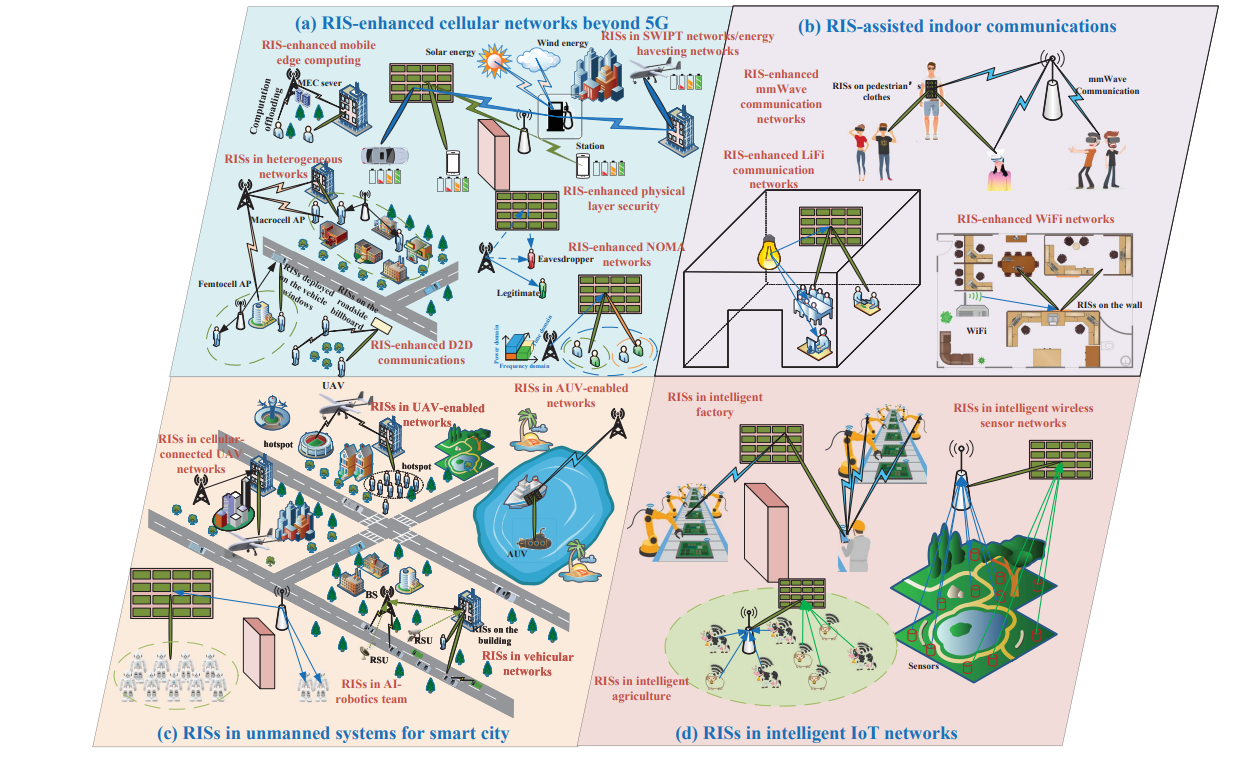
\includegraphics[width=14cm, height=8.5cm]{figures/RISusecases.png}
    \legend{Fonte: Produzido pelos autores}
  \end{minipage}
  \hfill

\end{figure}

\subsection{RIS como Antenas }  

Superfícies reconfiguráveis inteligentes são estruturas bem semelhantes aos arranjos de antenas, cujos elementos também são antenas. Pois na realidade toda superfície, até mesmo as dielétricas, são antenas irradiadoras de energia. O que as diferencia de uma “boa antena” são as propriedades requeridas de irradiação para uma determinada aplicação. No caso as RISs, são antenasr passivas ou ativas, terminadas em curto circuito, circuito aberto ou em uma impedância reativa cujo objetivo é direcionar, absorver, transmitir ou espalhar a energia eletromagnética de maneira controlada. De maneira análoga aos arranjos, ao modificar as impedâncias de cada elemento, intrinsecamente relacionadas à defasagem e à alteração da amplitude destes no âmbito do processamento digital e espacial dos sinais. Pode-se desenhar feixes segundo as necessidades requeridas para o usuário.

\subsection{RIS como Metasuperfícieis} 

O arranjos de elementos irradiadores são geralmente considerados metasuperficies (\textint{metasurfaces}). A metasuperfície pode ser considerada como uma estrutura bidimensional constituida de metamateriais, e pode realizar o controle da amplitude, fase e estado de polarização/direção da onda eletromagnética incidente. Metamaterial é um tipo de material ou estrutura que é projetado artificialmente e tem propriedades eletromagnéticas excepcionais e/ou outras propriedades físicas, não encontradas na natureza. AS metasuperfícies de \textit{Huygens} , 
Com base no princípio de Huygens e da generalização da lei de reflexão e refração de Snell, e do princípio da equivalência de Love, cada unidade com tamanho em em torno subcomprimento irá ser excitado por ondas eletromagnéticas incidentes com densidades de corrente superfíciais e gerar um pacote de ondas esféricas na interface metasuperfície/ar, podendo ser decomposta em um espectro de ondas planas e resolvidas separamente com a Lei de Snell. A onda esférica gerada por todas as unidades da metasuperfície formam uma nova frentes de ondas eletromagnética. 

\subsection{RIS, IRS ou LIS} 
    
Na literatura, parece não haver consenso, ou se visto por outro ponto de vista, várias definições são usadas para definir as superfícies inteligentes: superfícies reconfiguráveis inteligentes (RIS), superfícies refletoras inteligentes (IRS), meta-superfícies reconfiguráveis inteligentes, superfícies inteligentes longas (LIS) \cite{SDNRIS} . 

Na concepção destes autores até o presente momento, a RIS seria um termo geral para superfícies inteligentes, que aplicável a todos os tipos de funcionalidadeds. As meta-superfícies fazem alusão aos componentes, que majoritariamente são concebidos com metamateriais \cite{SREMetasurface}. Por outro lado as IRSs são como \textit{reflectarrays} (arranjos refletores) sendo atualmente utilizadas como antenas para aplicações em sistemas de satélites e outros sistemas de telecomunicações, moldando a reflexão. 

Portanto, decide-se empregar o termo RIS para o caso generalizado, e a terminologia IRS para o caso particular de reflexão. 

\section{ Classificações da RIS}

Existem diversas classificações para RIS quanto as suas características, como funcionalidade, tipo de elementos, espectro de frequência, arquitetura e tecnologias de reconfiguração.

\subsubsection{Funcionalidade} 

As classificações de funcionalidaeds são temas de grande debate. Em [] define-se a RIS híbrida refletora e de detecção (RIS \textit{Hybrid reflecting and sensing} - HRIS). Já para \cite{CFGOBDRIS}, RIS híbridas englobam o modo de transmissão e reflexão ao mesmo tempo. No nosso entendimento, uma RIS híbrida possui duas ou mais funções, não somente o caso convencional de reflexão. 
\begin{itemize}
   
    \item \textbf{Reflexão :} Refletem os sinais, podendo direcionar em determinada direçã ou espalhar em diversas direções;

    \item \textbf{Transmissão:} Transmitem o sinal, entretento, podem modificar a direção e formato do feixe que atravessa sua superfícies.


    \item  \textbf{Absorção:} Servem para absorver e/ou atenuar sinais indesejados, para diminuir interferência, segurança;

    \item \textbf{Detecção:} São ris que detecenão os sinais RF com o intuito de otimizar a aquisição de informação do canal. 

 \item  \textbf{Computação:} São RIS que podem funcionar como computadores analógicos e/ou digitais, realizando o processamento de informação.

 \item \textbf{Captura/Colheita:} Funcionam no modo de captura de energia, anlogamente as placas solares, porém para energia radiofrequência.

- Híbridas : Pode possuir 2 ou mais funcionalidades
\end{itemize}

\subsubsection{Elementos}   

\begin{itemize}

\item \textbf{Passivos:} Possuem elemetos sem elementos ativos, elementos que ocasionão a defasagem dos sinais eletromagnéticos, sem adicionar energia ao sistema.

\item \textbf{Ativos:} Possuem elementos ativos como amplificadores, para fortificar os sinais, porém não possuindo um cadeia radiofrequência completa como nos \textit{relays}.

\item \textbf{Híbrida:} Possuem os dois tipos de elementos.

\subsubsection{Bandas de Frequência} 

\item \textbf{Sub-6:} Frequências inferiores a 6 GHz. Nestas bandas, a RIS pode melhorar a cobertura, principalmente em regiões de penumbra causado por obstáculos, além de enriquecer ou atenuar o multipercurso para MIMO.

\item \textbf{Mid-Range:} Frequências entre 6-30 GHz, a atenuação começa ser um fator importante, pode auxiliar a desviar dos obstáculos e direcionar a energia para o usuário.

\item \textbf{Ondas milimétricas (mmWW), 30-300 GHz:} Atenução forte, combina uma boa largura de banda com uma certa capacidade de propagação em distâncias até revelantes de algumas centenas de metros. A diretividade da energia se torna cada vez mais importante.

\item Terahertz: Grande largura de banda tipo fibra ópitca, com atenução muito severa do sinal que não penetra objetos, pequena largura do feixe das ondas. Logo, superfícies largas podem relativisar esses efeitos. 
\end{itemize}

\subsubsection{Arquitetura} 

\begin{itemize}

Os autores de [] introduziram a interessante classificação da arquitetura em relação a caracteristica da matriz de espalhamento, cada elemento sendo como uma porta de uma rede radiofrequência.

\item \textbf{Elementos não são conectados entre si:} Comumente chamada de RIS com Matriz de Espalhamento Diagonal, pois os elementos não são conectados por conexões físicas controláveis e desejáveis. O autor também enumera outras subclassificações.

\item \textbf{Elementos conectados entre si por impedâncias:} Comumente chamada de Matriz de Espalhamento não diagonal, porque os elementos possuem conexões físicas controláveis e desejáveis. O autor também enumera outras subclassificações.

Porém, no desenvolvimento de RIS, os elementos estão conectados eletromagnéticamente pela Física mesmo que não esteja por conexões físicas como impedãncias controlladas, sendo na verdade a RIS naturalmente diagonal, contudo esses efeitos são desprezados, quando são desprezíveis, e/ou para facilitar o tratamento matemático. O método dos momentos justamente proporciona essa modelagem física completa, tratando e generalizando o sistema como não diagonal.

\end{itemize}

\subsubsection{Tecnologia de Reconfiguração } 

A tecnologias de reconfiguração são diversas, principalmente advindas das metasuperfícies, com tecnoloigias baseadas em semicondutores, dispositivos mecâncicos, quimicos ou termicos. Porém, focaremos nas tecnologias eletroeletrônicas.
\begin{itemize}
\item \textbf{Chaves (Transistors) :} Mais conhecidas como RF\textit{switches}.

 \textbf{Prós:} Preferido para aplicações que priorizam ampla largura de banda, alto isolamento e implementações de controle mais simples.
    
\textbf{Contras:} Sem o ajuste fino da formação de feixe.

   \textbf{Frequências de Operação:} Mais utilizado em frequências de até algumas dezenas de GHz, porém semicondutores que operam em ondas milimétricas, sub-THz e THz, estão em fase de pesquisa e maturação.
   
\item \textbf{Diodos Varactor}

    \textbf{Prós:} Adequado para aplicações que exigem formação de feixe precisa, ajuste fino de fases de sinal e baixo consumo de energia.

    \textbf{Contras:} Circuito de controle complexo.

    \textbf{Frequências de Operação:} Mais utilizado em frequências de até algumas dezenas de GHz, porém semicondutores que operam em ondas milimétricas e THz, estão em fase de pesquisa e maturação.


\item \textbf{Diodos PIN}

    \textbf{Prós:} Mais adequado para aplicações que exigem comutação rápida, alto isolamento ou controle de amplitude, como modelagem dinâmica de feixe ou comutação de frequência.

    \textbf{Contras:} Alto consumo de energia, baixa resolução do controle de fase e amplitude do feixe.

    \textbf{Frequências de Operação:} Mais utilizado em frequências de até algumas dezenas de GHz, porém semicondutores que operam em ondas milimétricas e THz, estão em fase de pesquisa e maturação.


\item \textbf{MEMS :} Não é uma tecnologia puramente mecânica, pois o controle se dá por comandos elétricos.

    \textbf{Prós:} Os MEMS oferecem alta precisão, devido boa linearidade e uma boa amplitude das faixas de mudança de mudança de fase. 

    \textbf{Contras:} Têm velocidades de comutação mais lentas e potenciais problemas de confiabilidade.

    \textbf{Frequências de Operação:} Frequências Microondas e sub-THz.

\item \textbf{Cristal líquido}

    \textbf{}\textbf{Prós:} Os cristais líquidos oferecem grandes faixas de mudança de fase e operação de banda larga, além de boa linearidade. 

    \textbf{Contras:} Têm velocidades de comutação mais lentas.

    \textbf{Frequências de Operação:} Frequências Microondas, sub-THz e THz.

\item \textbf{Grafeno: }

    \textbf{Prós:} O grafeno oferece potencial para desempenho superior em termos de capacidade de ajuste, largura de banda e velocidade de comutação.

    \textbf{Contras:}  A maturação da integração e da fabricação é ainda um  desafio.

    \textbf{Frequências de Operação:} Na faixa de THz é baseado no conjunto reativo/resitivo da impedância superficial. Porém, também pode ser usado em frequências inferiores, em microondas, baseado na parte resistiva da impedância superficial, especialmente como excelentes absorvedores banda larga.

\end{itemize}


\section{Modelagem Eletromagnética}\label{FormulaçãoPWTLBalanis}

A modelagem de superfíceis refletores inteligentes por teoria de circuitos elétricos e linhas de trnasmissão é similar a técnica comumente utilizada na literaturas para projetar as metasuperfícies. Por serem estruturas com espessura de sub-comprimento de onda, ou particulas polarizadas . Estas são tratadas matematicamente como uma fronteira entre dois meios, podendo ser vistas como impedâncias superficiais que provocam discontinuidades nos campos eletromagnéticos. Essas superfícies são definidas por alguns autores como Metasuperfícies de Huygens, um caso geral da natureza eletromagnética dos metamateriais, que com dimensions de sub-comprimnento de onda seguem o príncípio da equivalência  \cite{BalanisAEM}. Uma vez que com base no método das condições de fronteira eletromagnéticas , a natureza pode ser elétrica e magnética. Essas superfícies são tratadas como a superposição de dipolos eléricos e dipolos magnéticos que variam espacialmente e impõem discontinuidades eletromagnéticas superficiais entre dois meios \cite{GSTC}. Possibilitando a manipulação arbitrária do meio para diversas aplicações desde transformandores de feixes gassianos em feixes de bessel, capa de invisibilidade, controle arbitrário da direção e forma do feixe , antenas. Análise por circuitos elétricos e redes multiportas, também intrisecamente relacionada devido a dualidade com os campos eletromagnéticos.
Nesse âmbito como as RIS também são homonimamente denominadas metasuperfícies. O desenvolvimento por teoria de ondas planas é um técnica bastante utilizada \cite{BalanisAEM},\cite{EMPWTL}, onde o meio é considerado infinito, porém usado como aproximação para espessuras bem inferiores ao comprimento de onda.


\subsection{Definição dos Campos Eletromagnéticos}
\\
Para a RIS, de forma geral, que opere tanto em modo refletor quanto transmissor, como ilustrado na Fig. 1, representamos dois meios separados pela discontinuidade da IRS. O meio 1 em $z>0$, engloba os campos eletromagnéticos de incidência $\overline{E}_{i}(\theta_i,\phi_i)$ e espalhamento $\overline{E}_{i}(\theta_s,\phi_s)$, já o meio 2, em $z<0$, o campo eletromagnético transmitido neste . Logo define-se os campos elétricos como,\\
\begin{equation}
      \overline{E}_{1}=\overline{E}_{i}
      +\overline{E}_{s}, \ \ z > 0\\
\end{equation}
\begin{equation}
       \overline{E}_{2} \   \ z < 0 \\
\end{equation}
\begin{equation}
      \overline{H}_{1}=\overline{H}_{i}
      +\overline{H}_{s}, \ \ z > 0\\
\end{equation}
\begin{equation}
       \overline{H}_{2}\   \ z < 0 \\
\end{equation}

As condições de fronteira eletromagnéticas nos dão a seguintes relaçãos para os campos elétromgnéticos

\begin{equation}{\label{BoundaryFields}}
 [(\overline{E}_s+\overline{E}_{i})\cdot \overline{a}_t]\overline{a}_t=E_2
\end{equation}
\begin{equation}{\label{BoundaryFieldsImp}}
 [(\overline{E}_s+\overline{E}_{i})\cdot \overline{a}_t]\overline{a}_t=Z_s\overline{J}_{s}
\end{equation}
\begin{equation}{\label{BoundaryCurrent}}
  \overline{a}_z  \times [{\overline{H}_{2}-\overline{H}_{1}} ]=\overline{J}_{s}
\end{equation}

\subsection{Modelagem pelas Equações de Espaço Livre}\label{FormulaçãoFreeSpace
Balanis}

A propagação no espaço livre, no campo distante, é largamente utilizada e descrita pela equação Fris. Porém, sendo necessária a obtenção dos parâmetros de ganho das antenas, área efetivas e potência de transmissão. Os dois primeiros obtidos geralmente por simulações numéricas das antenas. Por outro lado para cenários de espalhamento e de propagação mais complexa, a física ótica e/ou traçado de raios (ray tracing) é amplamente empregado pelos pesquisadores e engenheiros.

Dentro deste contexto, deriva-se a potência e eficiência espectral para um único usuário, uma IRS único transmissor (podendo ser um arranjo de antena) utlizando a equação de Fris {[}27{]}. Inferindo as potências
recebidas a partir da área efetiva e do radar cross section da IRS que cálcularemos com o método dos momentos. Portanto, a densidade de potência incidente a partir do transmissor direcionada ao usúario e à IRS são, respectivamente, descritas por,

\begin{equation}
W_{txk} = W_{0txk}G_{txk} = \frac{P_{t}G_{t}(\theta_{txk},\phi_{txk})}{(4\pi R_{1}^{2})}
\end{equation}
\begin{equation}
    W_{txirs} = W_{0txirs}G_{txirs} = \frac{P_{t}G_{t}(\theta_{txirs},\phi_{txirs})}{(4\pi R_{2}^{2})}
\end{equation}




Define-se como $\lambda$ o comprimento de onda,
$G_{txk} = G_{t}(\theta_{txk},\phi_{txk})$ o ganho da antena transmissora na direção do usuário,
$G_{txirs} = G_{t}\left( \theta_{txirs},\phi_{txirs} \right)$ o ganho da antena transmissora na direção da IRS, $G_{r}(\theta_{rxtx},\phi_{rxtx})$ o ganho da antena do usuário na direção do transmissor, $A_{rxtx}$ a área efetiva do usuário na direção do transmissor, $P_{t}$ a potência de transmissão, $R_{1}$ a distância entre o transmissor e o usuário, e $R_{2}$ a distância entre o transmissor e a IRS. Logo, a potência recebida diretamente pelo usuário diretamente do AP é,

\begin{equation}
    P_{tx - user} = W_{txk}A_{rxtx} = \frac{P_{t}G_{t}\left( \theta_{txk},\phi_{txk} \right)G_{r}\left( \theta_{rxtx},\phi_{rxtx} \right)\lambda^{2}}{\left( 4\pi R_{1} \right)^{2}}
\end{equation}


A área efetiva da IRS e do usuário receptor para o feixe advindo da IRS são dadas, respectivamente, como
\begin{equation}
A_{irs} = \sigma_{irs}(\theta_{irs},\phi_{irs})
\end{equation}


\begin{equation}
A_{rxirs} = \left( \frac{\lambda^{2}}{4\pi} \right)G_{r}\left( \theta_{rxirs},\phi_{rxirs} \right)\ 
\begin{equation}


Sendo $\sigma_{irs}(\theta_{irs},\phi_{irs})$, o \emph{radar crosssection} da IRS na direção do usuário,
$G_{r}\left( \theta_{rxirs},\phi_{rxirs} \right)$  O ganho da antena na direção do feixe advindo da IRS. Obtem-se a potência recebida pela IRS para a distância $R_{1}$ entre o transmissor e a IRS, como,

\begin{equation}
    P_{irs} = W_{txirs}A_{irs} = \frac{P_{t}G_{t}(\theta_{txirs},\phi_{txirs})}{(4\pi R_{2}^{2})}\sigma_{irs}\left( \theta_{irs},\phi_{irs} \right)
\end{equation}

Analogamente, define-se a densidade de potência da onda espalhada pela IRS na direção do usuário por uma distância $R_{3}$,
\begin{equation}
    W_{s} = \frac{P_{irs}}{(4\pi R_{2}^{2})} = \frac{P_{t}G_{t}(\theta_{txirs},\phi_{txirs})}{\left( 4\pi R_{2}R_{3} \right)^{2}}\sigma_{irs}\left( \theta_{irs},\phi_{irs} \right)
\end{equation}

Deste modo, a potência recebida pelo usuário através da IRS é dada,
\begin{equation}
    P_{tx-irs-user} = A_{rxirs}W_{s}
\end{equation}
\begin{equation}
    P_{tx - irs - user} = \sigma_{irs}\left( \theta_{irs},\phi_{irs} \right)\frac{P_{t}G_{t}(\theta_{txirs},\phi_{txirs})G_{r}\left( \theta_{rxirs},\phi_{rxirs} \right)}{4\pi}\left( \frac{\lambda}{4\pi R_{2}R_{3}} \right)^{2}
\end{equation}

Portanto a potência total do usuário,

\begin{equation}
    {P_{rxtotal} = P_{tx -user} + P}_{tx-irs-user}
\end{equation}

\begin{equation}
    P_{rxtotal} = \frac{P_{t}G_{t\ }\left( \theta_{txk},\phi_{txk} \right)G_{r}\left( \theta_{rxtx},\phi_{rxtx} \right)\lambda^{2}}{\left( 4\pi R_{1} \right)^{2}} + \\
\sigma_{irs}\left( \theta_{irs},\phi_{irs} \right)\frac{P_{t}G_{t}(\theta_{txirs},\phi_{txirs})G_{r}\left( \theta_{rxirs},\phi_{rxirs} \right)}{4\pi}\left( \frac{\lambda}{4\pi R_{2}R_{3}} \right)^{2}
\end{equation}

A eficiência espetral é dada por,

\begin{equation}
SE = \left( 1 - \frac{1}{3850} \right)\log_2\left( 1 + \frac{P_{rxtotal}}{N_{\sigma}} \right)    
\end{equation}

Se considerarmos o temperatura das antennas ( os elementos da RIS) e do sistema, temos a potência do ruído, como

\begin{equation}
  N_{\sigma - dB} = 10\log{\left( KT_{s}B \right) =}10{\log{\left( KT_{a}B \right) + NF}}_{dB}  
\end{equation}
\begin{equation}
    T_{s} = T_{a\ } + T_{rx}
\end{equation}

Assumindo $T_{s}$ como a temperatura do sistema, $T_{a\ }$ a temperature da antenna, $T_{rx}$ temperatura do receptor radiofrequência do usuário, $K$ a constante de Boltzmann e B a largura de banda do sinal.


\subsection{Modelagem pelo Método de Arranjo de Antenas}\label{FormulaçãoArrayBalanis}

Os método de arranjos é um clássico que nunca sai de moda, comumente usado na literatura para analisar arranjos de antenas perfeitos, sem considerar todos os efeitos eletromagnéticos reais, com o intuito de construir diagramas ideais e perfeitos de referência que guiam a modelagem dos arranjos para uma determinada aplicação, com uma determinada técnica de atribuição dos pesos complexos. Por exemplo, a amplitudes e fase dos sinais são modificados pelos amplificadores, defasadores, pelos coeficientes de reflexão complexos dos elementos da RIS. Portanto, a RIS também pode ser vista como um arranjo de antenas, que ao refletir aplica um peso complexo a amplitude do campo elétromagnético da onda incidente.

Considerando um arranjo planar distribuido no plano $xy$, com $N_{ZsW}$ elementos em x, com $N_{ZsL}$ elementos em y, 

\textbf{
Fig. Fazer Figura}


O modelo planar do método de arranjo de antenas clássico {cite}`balanisAntenna` é dado por

\begin{equation}
    \overline{E}_s=\sum_{m=1}^{M} \sum_{n=1}^{N} I_{1m}e^{j(m-1)kd_x \sin \theta \cos \phi+\Omega_x}
                                I_{1n}e^{j(m-1)kd_x \sin \theta \cos \phi+\Omega_x}
\end{equation}

Sendo que $\beta_x$ e $\beta_y$, são a defasagens continuamente aplicadas, respectivamente,  aos elementos ao longo dos eixos $x$ e $y$.
Porém se considerarmos coeficiente de reflexão com amplitude e fase variável ao longo de todo os, a defasagem entre elementos vizinhos, podendo não ser necessariamente constante. O coeficients de reflexão da RIS paras as duas polarizações

\begin{equation}
\Gamma^{x}_{NM}=A^{x}_{NM} e^{j \Omega^x_{NM}}e^{j \Omega^y_{NM}}
\end{equation}

\begin{equation}
\Gamma^{y}_{NM}=A^{y}_{NM} e^{j \Omega^x_{NM}}e^{j \Omega^y_{NM}}
\end{equation}

O coefiente englobando o efeito das duas componentes,

\begin{equation}
\Gamma_{NM}=\Gamma^{x}_{NM}\Gamma^{y}_{NM}=A_{NM} e^{j \Omega^x_{NM}}e^{j \Omega^y_{NM}}
\end{equation}


Logo, considerando a RIS de referência, o campo incidente sendo unitário e em phase sobre toda a superfície 
\begin{equation}
\overline{E}_s=\sum_{m=1}^{M} \sum_{n=1}^{N} A_{NM}e^{j(m-1)kd_x \sin \theta \cos \phi+\Omega_{NM}^x}
                                e^{j(m-1)kd_x \sin \theta \cos \phi+\Omega_{NM}^y}
\end{equation}

\subsection{Modelagem pelo Método de Ondas Planas e Linhas de Transmissão}\label{FormulaçãoPWTLBalanis}
Método de ondas planas, também um clássico e extraordinário, uma vez que todo campo eletromagnético pode ser decomposto em um espectro de ondas planas, se o divergente do camplo eletromagnético for zero, tratando o problema também no espaço spectral dos ângulos, direções das ondas incidentes, ele analisa as reflexões e transmissões de ondas planas entre diferentes meios, levando conta suas características dos meios a partir das impedâncias das ondas eletromagnéticas nos respectivos meios. 

O método das Linhas de transmissão também compartilha a mesma essência do método de ondas plans, mas neste método se dá com a manipulação das impedâncias e parâmetros de circuitos elétricos, tendo também muita importância no desenvolvimento dos ciruitos eletromagnéticos das antenas, como o a optimização do casamento de impedâncias, pode-se tratar todo o sistema de irradiação como um circuito elétrico.

Logo, tem-se a visão tanto espaço espectral ângular como do espaço spectral frequencial, assim como a modelagem por circuitos elétricos.

\subsubsection{Descrição do Método}  

Neste método, considera-se uma onda incidente que se propaga na linha de transmissão do ar, e alcança uma discontinuidade, representada por uma impedância superficial $Z_s$, que representa a RIS. Essa impedância irá espalha um campo eletromagético, assim como transmitir outro campo eletromagnético na linha de transmissão do ar.

<img src="https://external-content.duckduckgo.com/iu/?u=http%3A%2F%2Fdrive.google.com/uc?id=1i2FgcvuscNZaELtdCInN_5nCSkCVawbb" 
    style="width: 300px;  height: 300 px;display: block;margin-left: auto;margin-right: auto;"  />
Dadas as condiçõoes de contorno e a definição dos campoes \cite{A}, a impedância vista da RIS representada pela impedância superficial e o meio 2 que pode ser considerada uma linha de transmissão, é dada por,

\begin{equation}{\label{ImpedanciaZinParaleloZsEta2}}
   Z_{in}= \frac{Z_s \eta_2^{TM} }{\eta_2^{TM}+Z_s}
\end{equation}
Se o meio 2 é o idêntico ao meio 1, e todos os dois, o espaço Livre, o caso da RIS, pois a impedância superficial encapsula toda estrutura, temos $\eta^{TM}_{2}=\eta^{TM}_1=\eta^{TM}_0$

E o coeficiente de reflexão se deduz como,
\begin{equation}
   \Gamma= \frac{Z_{in}-\eta_1^{TM}}
    {Z_{in}+\eta_1^{TM}}
\end{equation}
Se os dois meios forem o espaço livre,
\begin{equation}
    \Gamma=\frac{-\eta^{TM}_0}{2Z_s+\eta^{TM}_0}
\end{equation}

A impedância superficial em relação ao coeficiente de reflexão

\begin{equation}
    Z_s=\frac{\eta^{TM}_0(1+\Gamma)}{2\Gamma}
\end{equation}

\subsection{ Modelagem Circuito elétrico}#

O circuito básico dá RIS pode ser modificado em relação ao descrito anteriomente, identificando melhor as estruturas do sistema, entrando mais no conceito dos circuitos elétricos com suas resistências, capacitâncias e indutâncias. Que se constitue geralmente de um \textit{patch} sob um substrado dielétrico com um plano de terra na sua superfície inferior. Nesta nova configuração, a onda incidente encontra primeirammente impedância do \textit{patch}  $Z_p$ e logo após percorre a linha de trasmissão do dielétrico com impedância de onda $\eta_d$ que está curto circuitada pelo plano de terra de impedância $Z_g$.

Melhorar figura e colocar Zg (exportar, não faz )
<img src="https://external-content.duckduckgo.com/iu/?u=http%3A%2F%2Fdrive.google.com/uc?id=17_eq7NOBCh6Q9ycTYJQGyD6bm6H1CCQd" 
    style="width: 300px;  height: 300 px;display: block;margin-left: auto;margin-right: auto;"  />
Do \textit{patch} tem-se $Z_p$,

\begin{equation}
Z_p=R_p+j\omega L_p+\frac{1}{j\omega C_p}
\end{equation}
No dominio de Laplace

\begin{equation}
Z_p(s)=\frac{sR_p+s^2 L_p+1/C_p}{s }
\end{equation}

Sendo $R_p$ a sua resistência superfical, $C_p$ a sua capacitância, $L_p$ a sua indutância. Já para o dielétrico, a impedância vista a partir do \textit{patch} é dada por


\begin{equation}
Z_d=\eta_d\frac{Z_g+j\eta_d \tan{kl}}{\eta_d+jZ_g\tan{kl}}
\end{equation}

Como $ Z_g$ é muito pequena, tem-se

\begin{equation}
Z_d=j\eta_d\tan{kl}=jX_d
\end{equation}
No dominio de Laplace
considerando a variação da indutância bem pequena com a frequência

\begin{equation}
Z_d(s)=s L_d
\end{equation}
 
A impedância vista pela onda incidente, será

\begin{equation}
   Z_{in}= \frac{Z_p Z_d}{Z_p+Z_d}
\end{equation}


Se todo circuito for encapsulado como descrito inicialmente, em uma impedância $Z_s$, teremos

\begin{equation}
    Z_s=\frac{Z_{in}\eta_0^{TM}}{\eta_0^{TM}-Z_{in}}
\end{equation}

Porém analisando melhor,

\begin{equation}
   Z_{in}= \frac
   {(\frac{sR_p+s^2 L_p+1/C_p}{s }) (sL_d)
   }
   {
  (\frac{sR_p+s^2 L_p+1/C_p}{s })+sL_d
   }
\end{equation}

\begin{equation}
   Z_{in}= \frac
   {
      (sR_p L_d+s^2 L_pL_d+L_d/C_p)s
   }
   {
      sR_p+s^2 L_p+1/C_p+s^2L_d
   }
\end{equation}

\chapter{Formulação do MoMCSL}\label{FormulaçãoMoMCSL}


Nesse capítulo desccreveremos a formulação matemática e física do método dos momentos (MoM). A implementação matemática e os cálculos numéricos serão realizados usando o programa comercial Matlab. As IRSs, por serem estruturas planares, optou-se pelo método dos momentos bidimensional (MoM-2D) para analisar numericamente como realizado por Costa e Dmitriev . 
espaçamento menor que meio comprimento de onda [Balanis][Phased array]. Além da espessura 3 D dos elementos serem menores que o comprimento de onda, toda estrutura pode ser aproximada por uma impedância de superfície. Como a impedância pode ser negativa, contudo o coeficiente de cada elemento sendo menor que 1, pode se alcançar uma resolução de fase de 360 Graus para os  \emph{phase shifters}. Este chamaremos de MoMCSL (MoM continous and single Layer). Este método utiliza as equações do vetor magnético pontecial $\overline{A}$ e do potencial escalar elétrico $\phi$ em seu desenvolvimento, advindas das equações de Maxwell. Apesar da última também poder ser escrita em função da densidade corrente ou do potencial magnético A. Tem-se a semântica de que fazendo a separação das duas, a primeira representa a lei de faraday da indução, no qual os campos eletromagnéticos variantes no tempo rotacionam, o mais representativo da propagação no campo distante, e a segunda, a lei de Gauss da concentração de cargas encerradas por determinada superfície, para o qual os campos não dirvergem ou convergem ao/do infinito, característico do campo próximo, onde há descontinuidades das linhas de campo e das condições de contorno. Logo as seguintes formulações são usadas


\begin{equation}{\label{CampoEspalhado}}
  \overline{E}_{s}=-j\omega \overline{A} - \nabla \Phi
\end{equation}
\begin{equation}{\label{VetorPotencialMagnetico}}
  \overline{A} =\mu \iint\limits_S\overline{J} \frac{e^{-j k R}}{4 \pi R} dS^{'}
  \end{equation}
\begin{equation}{\label{PotencialEscalar}}
  \Phi =-\frac{1}{j\omega \epsilon}\iint\limits_S \nabla \cdot \overline{J}\frac{e^{-j k R}}{4 \pi R} dS^{'}
  \end{equation}
Considerando $R=|\overline{p}-\overline{p^{'}}|$,  se $\overline{p}$ é o vetor posição de um determinado ponto na superfície  analisado e $\overline{p^{'}}$ o vetor posição do conjundo de pontos na superfície $S$, somados um a um. A superfície $S$ pode ser a união de várias surperfícies distintas, de várias IRS e/ou conjunto de antenas. Fica implícito que a densidade de corrente superficial $\overline{J}$ depende de $\overline{p}$ e $\overline{p^{'}}$. 

\section{MoM com Impedância Superficial}

Os parâmetros eletromagnéticos do material da IRS são encapsulados na impedância superficial $Z_s$. A seguinte condição de contorno dos campos elétricos deve ser respeitada:
  \begin{equation}{\label{CondiçãoDeContorno}}
    [(\overline{E}_s+\overline{E}_{i})\cdot \overline{a}_t]\overline{a}_t=Z_s\overline{J}
  \end{equation}
sendo $\overline{E}_i$ ($V/m^2$) é o vetor campo elétrico incidente proveniente de uma fonte distante, e que conhecemos sua intensidade na superfíe da IRS. Como a equação do vetor campo espalhado $\overline{E}_s$ resulta de uma operação linear  sobre a densidade de corrente, substituido o \ref{VetorPotencialMagnetico}-\ref{PotencialEscalar} em \ref{CampoEspalhado}
\begin{equation}
    \overline{E}_s \cdot \overline{a}_t=L_s(\overline{J})
\end{equation}
  \begin{equation}{\label{OperadorLinearCampoEspalhado}}
      L_s(\overline{J})= -j\omega \mu \iint\limits_S\overline{J} \frac{e^{-j k R}}{4 \pi R} dS^{'} +
    \nabla \biggl[ \frac{1}{j\omega \epsilon}\iint\limits_S \nabla \cdot \overline{J}\frac{e^{-j k R}}{4 \pi R} dS^{'}  \biggl] 
  \end{equation}
Além disso, a geometria da superfície e sua impedância superficial é predefinida. Temos a densidade de corrente $\overline{J}$ como variável não conhecida. Sabendo que $E_s$ depende da densidade de corrente, da geometria,  da permeabilidade magnética  $\mu_0$ e da permissividade elétrica $\epsilon_0$, ambas no espaço livre. As caracteristicas eletromagnéticas são unicamente definidas pela impedância superficial $Z_s$. Substituido a eq. \ref{OperadorLinearCampoEspalhado} em eq. \ref{CondiçãoDeContorno}
\begin{equation}
\overline{E}_{i}\cdot \overline{a}_t=Z_s\overline{J}+j\omega \mu \iint\limits_S\overline{J} \frac{e^{-j k R}}{4 \pi R} dS^{'} -
    \nabla \biggl[ \frac{1}{j\omega \epsilon}\iint\limits_S \nabla \cdot \overline{J}\frac{e^{-j k R}}{4 \pi R} dS^{'}  \biggl] 
\end{equation}
Temos as componentes $E_x^{i}$ e $E_y^{i}$ do campo incidente,

\begin{equation}{\label{CampoExTangencialEmFunçãoJ}}
  E_{x}^i=Z_s \overline{J}\cdot \overline{a}_x+j\omega \mu \iint\limits_S \overline{J}\cdot \overline{a}_x\frac{e^{-j k R}}{4 \pi R} dS^{'} -
     \frac{\partial }{\partial x}  \biggl[ \frac{1}{j\omega \epsilon}\iint\limits_S  (\frac{\partial J_x}{\partial x}+ \frac{\partial J_y}{\partial y} ) \frac{e^{-j k R}}{4 \pi R} dS^{'}  \biggl] 
\end{equation}
\begin{equation}{\label{CampoEyTangencialEmFunçãoJ}}
  E_{y}^i=Z_s \overline{J}\cdot \overline{a}_y+j\omega \mu \iint\limits_S \overline{J}\cdot \overline{a}_y \frac{e^{-j k R}}{4 \pi R} dS^{'} -
     \frac{\partial }{\partial y}  \biggl[ \frac{1}{j\omega \epsilon}\iint\limits_S  (\frac{\partial J_x}{\partial x}+ \frac{\partial J_y}{\partial y} ) \frac{e^{-j k R}}{4 \pi R} dS^{'}  \biggl] 
\end{equation}

Apesar dos resultados na maioria das vezes se intensificar no campo distante, podendo o potencial escalar ser desprezado se a excitação é conhecida. Observa-se que a interação entre os elementos no campo próximo interfere diretamente na corrente de excitação, assim como as componentes ortogonais de excitação dependem uma da outra, o que não é considerado em outros métodos comumente utilizados. O valor da corrente utilizada é considerado ideal, sem conter o efeito de sua vizinhança de campo próximo.
O procedimento do MoM tradicional enseja a expansão da solução em termos funções base . Além da realização do produto interno com uma função teste $w_m$ em ambos os lados da equação, no lado com as operações lineares sobre a solução, e no lado com o valor imposto ao resultado da operação linear, neste problema, o campo incidente.

\begin{equation}{\label{DefiniçãoProdutoInternoMoM}}
    \langle w_m,\overline{E}_i \rangle=  \langle w_m,Z_s\overline{J}-L_s(\overline{J})\rangle
\end{equation}
Se transformarmos o lado direito da equação \ref{DefiniçãoProdutoInternoMoM} em um operador linear $L=Z_s -L_s$ 
\begin{equation}{\label{DefiniçãoProdutoInternoLMoM}}
 \langle w_m,\overline{E}_i \rangle=  \langle w_m,L(\overline{J})\rangle
\end{equation}

Com o intuito de resolver o sistema linear de equações, transforma-se em um sistema matricial com uma matriz impedância reacionando a densidade de corrente e com a tensão incidente. A densidade de corrente depende  do acoplamento mútuo de cada elemento, incluíndo o efeito entre si das densidades de correntes ortogonais provenientes do potêncial escalar. 

Portanto temos, a tensão pode ser escrita na forma matricial
\begin{equation}
  [\Delta V_J]_{N_t \times 1} =\{ [Z_{s}^J\Delta l_J]-[Z_{JI}]\}_{N_t \times N_t}\times[J_I]_{N_t \times 1}
\end{equation} 
e a densidade de corrente,
\begin{equation}
  [J_I]_{N_t \times 1}=\{ [Z_{s}^J\Delta l_J]-[Z_{JI}]\}^{-1}_{N_t \times N_t} \times[\Delta V_J]_{N_t \times 1} 
\end{equation} 
Se representarmos com matrizes de acomplamento  para vizualizar, o  efeito do vetor potencial magnético representada pela matriz$[M]$ do vetor magnético e pela matriz $[C]$ o efeito potencial escalar das cargas  portando o acoplamento das polarizações.
\begin{equation}
\begin{aligned}
  \begin{bmatrix} [J^{x}_I]_{N_{xx}\times 1} \\ [J^{y}_I]_{N_{yy}\times 1}\end{bmatrix}  =\Biggl\{\begin{bmatrix}[Z_s^{xx}\Delta l_J]_{N_{xx}\times N_{xx}}& [O]_{N_{xx}\times N_{yy}}\\
   [O]_{N_{yy}\times N_{xx}}&[Z_s^{yy}\Delta l_J]_{N_{yy}\times N_{yy}}
   \end{bmatrix} 
   \\+
   \begin{bmatrix}[M_{JI}^{xx}]_{N_{xx}\times N_{xx}}& [O]_{N_{xx}\times N_{yy}}\\
   [O]_{N_{yy}\times N_{xx}}&[M_{JI}^{yy}]_{N_{yy}\times N_{yy}}
   \end{bmatrix}+
   \begin{bmatrix}[C_{JI}^{xx}]_{N_{xx}\times N_{xx}}& [C_{JI}^{xy}]_{N_{xx}\times N_{yy}}\\
   [C_{JI}^{yx}]_{N_{yy}\times N_{xx}}&[C_{JI}^{yy}]_{N_{yy}\times N_{yy}}
   \end{bmatrix} \Biggl\}^{-1}
\begin{bmatrix}[\Delta V^{x}_J]_{N_{xx}\times 1} \\ [\Delta V^{y}_J]_{N_{yy}\times 1}\end{bmatrix}
   \end{aligned}
\end{equation}

Como o campo a tensão do campo espalhado é expressa

\begin{equation}
  [\Delta V^s_J]_{N_t \times 1}= [Z_{IJ}]_{N_t \times N_t} [J_I]_{N_t \times 1} 
\end{equation}

 A matriz de acoplamento ou de parametros de espalhamento pode ser escrita como

\begin{equation}
  [S_{JJ}]_{N_t \times Nt}= [Z_{JI}]_{N_t \times N_t} [Y_{IJ}]_{N_t \times N_t}
\end{equation}



 \subsection{Disposição da RIS}
RIS tem $N_{ZsL} \times N_{ZsW}$ elementos na superfície $S$, porém cada antenna da IRS terá $N_{xZs}$ discretizações em $x$ e $N_{yZs}$ discretizações em $y$.  Logo temos
\begin{equation}
    N_{x}=N_{xZs}N_{ZsL}
\end{equation}
\begin{equation}
    N_{y}=N_{yZs}N_{ZsW}
\end{equation}
 Como na prática teriamos $N_{ZsL} \times N_{ZsW}$ impedâncias superficiais para as correntes $J_x$ e  $N_{ZsL} \times N_{ZsW}$ impedâncias superficiais para as correntes $J_y$.
Porém o MoM devido as eq. diferenciais do potencial escalar, as densidade de corrente $J_x$ tem $N_{x}-1$ linhas de discretização, se aplicarmos a impedância superfície diretamente nas formulação, A superfície ficaria diferente da desejada. Na verdade o tamanho dos elementos ficaria assimétrico.
 tem $N_{ZsL} \times N_{ZsW}$ elementos na superfície $S$, porém cada antenna da IRS terá $N_{xZs}$
\begin{equation}
    N_{x}=N_{xZs}N_{ZsL}
\end{equation}
\begin{equation}
    N_{y}=N_{yZs}N_{ZsW}
\end{equation}
 Como na prática teriamos $N_{ZsL} \times N_{ZsW}$  
 
\subsection{Far-Field Approximation}



A aproximação de campo distante é realizada de acordo com o Balanis, o campo elétrico em termos de coordenadas esféricas é escrito como,

 \begin{equation}
\begin{aligned}
E_{\theta}=-\frac{jk \eta e^{-j kR}}{4\pi R} 
  \iint \limits_S [J_x \cos{\theta} \cos{\phi}+J_y \cos{\theta} \sin{\phi}] dS^{'}
   \end{aligned}
\end{equation}
 \begin{equation}
\begin{aligned}
E_{\phi}=-\frac{jk\eta e^{-jkR}}{4\pi R} 
  \iint \limits_S [-J_x  \sin{\phi} +J_y \cos{\phi} ] dS^{'}
   \end{aligned}
\end{equation}
O espalhamento será avaliado em termos de seção reta radar ou \emph{radar cross section} (RCS), 

 \begin{equation}
\begin{aligned}
\sigma_{\theta}=4\pi R^2\frac{|E_{\theta}^s|^2}{|E_{\theta}^{i}|^2}=
\frac{\eta^2 k^2}{4 \pi}|Vr|
   \end{aligned}
\end{equation}










% ---
% primeiro capitulo de Resultados
% ---


\chapter{Resultados Numéricos}
Neste capitulo vamos analisar primeiramente a validade do nosso método numérico, parâmetros de malha e convergência. Primeiro, validamos nosso modelo com CST e AFM, depois realizamos o direcionamento do feixe para uma variação de fase na direção x.


\section{Validação da Malha}
A validação da malha é realizada comparando com o AFM [10], que é muito semelhante aos resultados da óptica física, e do CST. Os resultados numéricos do nosso modelo estão muito bem com as saídas CST e AFM conforme mostrado na Fig. 4, para planos de corte xoz e yoz relacionados à origem o. Consideramos uma placa quadrada de 5λ×5λ, em 3,3GHz, composta apenas por um condutor elétrico perfeito (PEC), portanto Z_(N,M)=0 sobre toda a incidência normal da superfície, ou seja, E_i (θ_i=0,ϕ_i =0).


\begin{figure}[htb]
 \label{DiscretizaçãoXY}
    \centering
    \caption{Ilustração da discretização  com a função base pulso} \label{fig_minipage}
    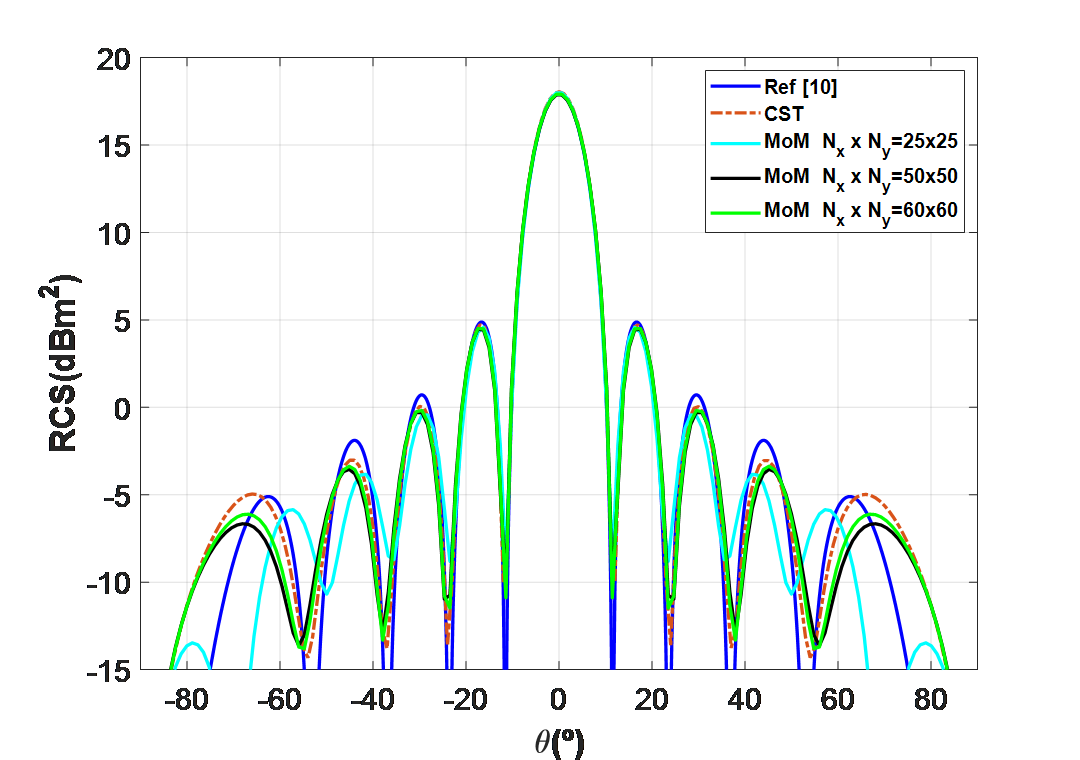
\includegraphics[width=\textwidth]{figures/RCSMeshValidationXoz.png}
    \legend{Fonte: Produzido pelos autores}
  \hfill
\end{figure}

\begin{figure}[htb]
 \label{DiscretizaçãoXY}
    \centering
    \caption{Ilustração da discretização  com a função base pulso} \label{fig_minipage}
    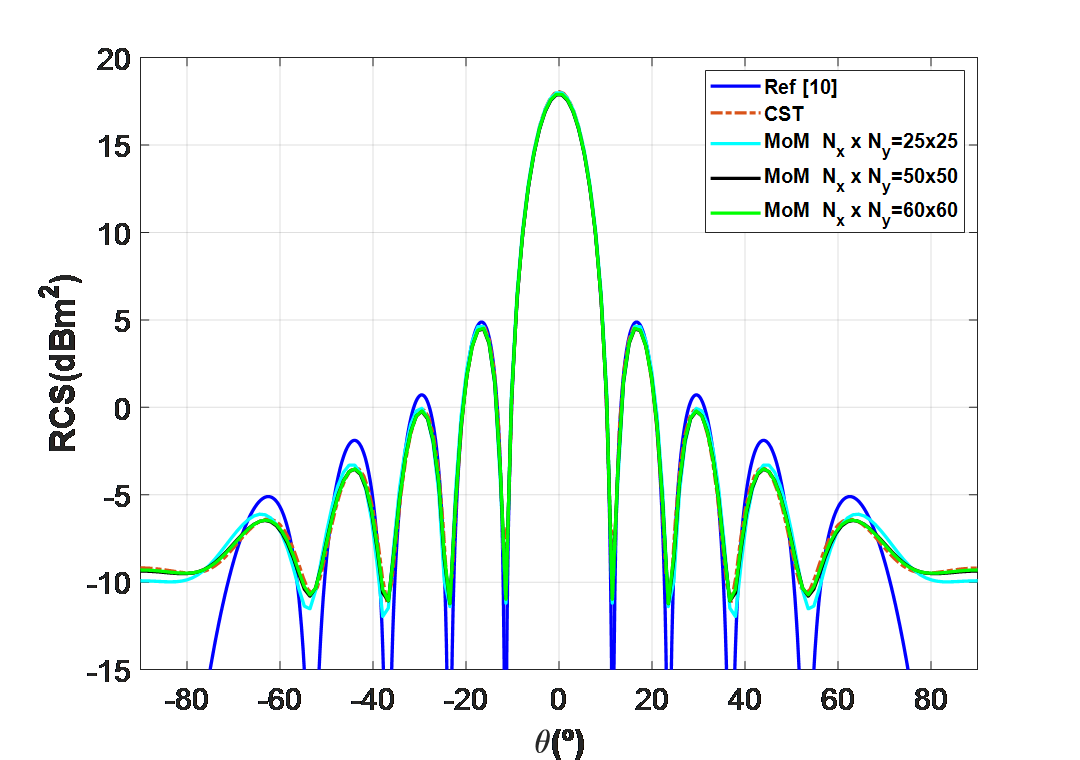
\includegraphics[width=\textwidth]{figures/RCSMeshValidationYoz.png}
    \legend{Fonte: Produzido pelos autores}
  \hfill
\end{figure}

Para analisar o espalhamento de controle do feixe, típico de aplicações reais de IRS, conforme eq. (4), a incidência normal também é presumida. Aplicamos uma sintonia de fase apenas na direção x em 5 e 10 impedâncias diferentes, escolhendo a direção alvo como $(\theta_s,_\phi_s=0)$ e mantendo a mesma área da seção anterior, $N_ZsW=1$ e $N_yZs=50$. A discretização da malha é mostrada na Fig. 5. 


\begin{figure}
\centering
\begin{subfigure}{.5\textwidth}
  \centering
  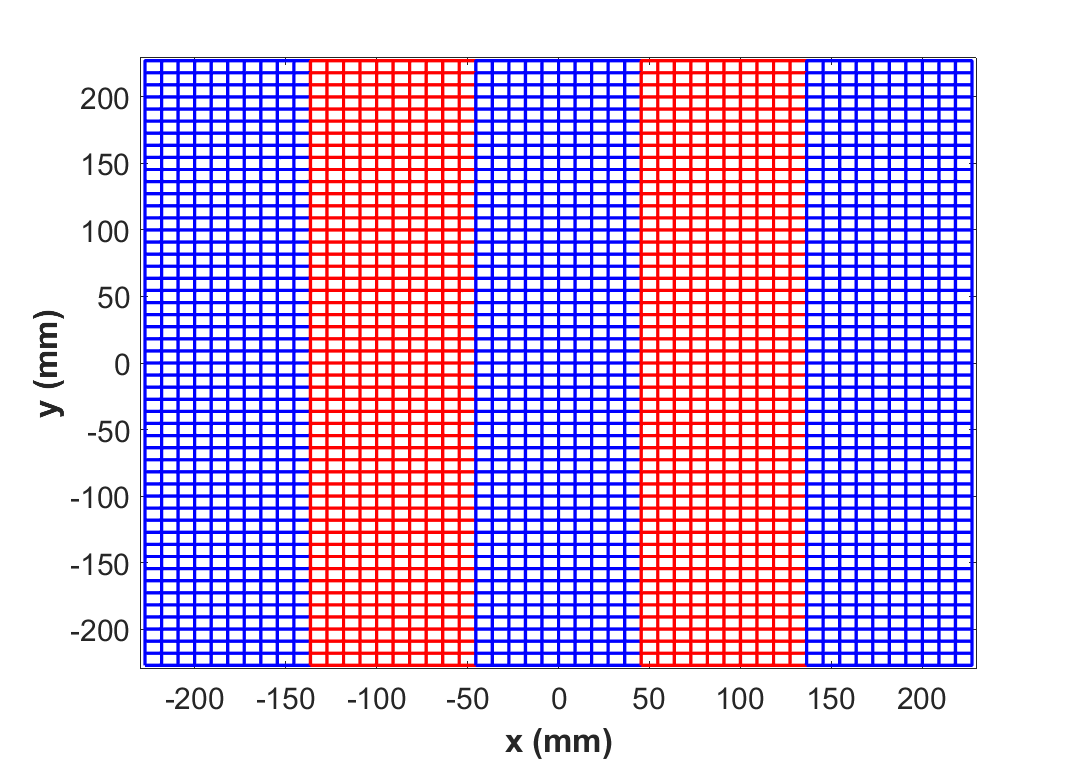
\includegraphics[width=\textwidth]{figures/MeshDiscretization5.png}
  % \caption{A subfigure}
  \label{fig:sub1}
\end{subfigure}%
\begin{subfigure}{.5\textwidth}
  \centering
  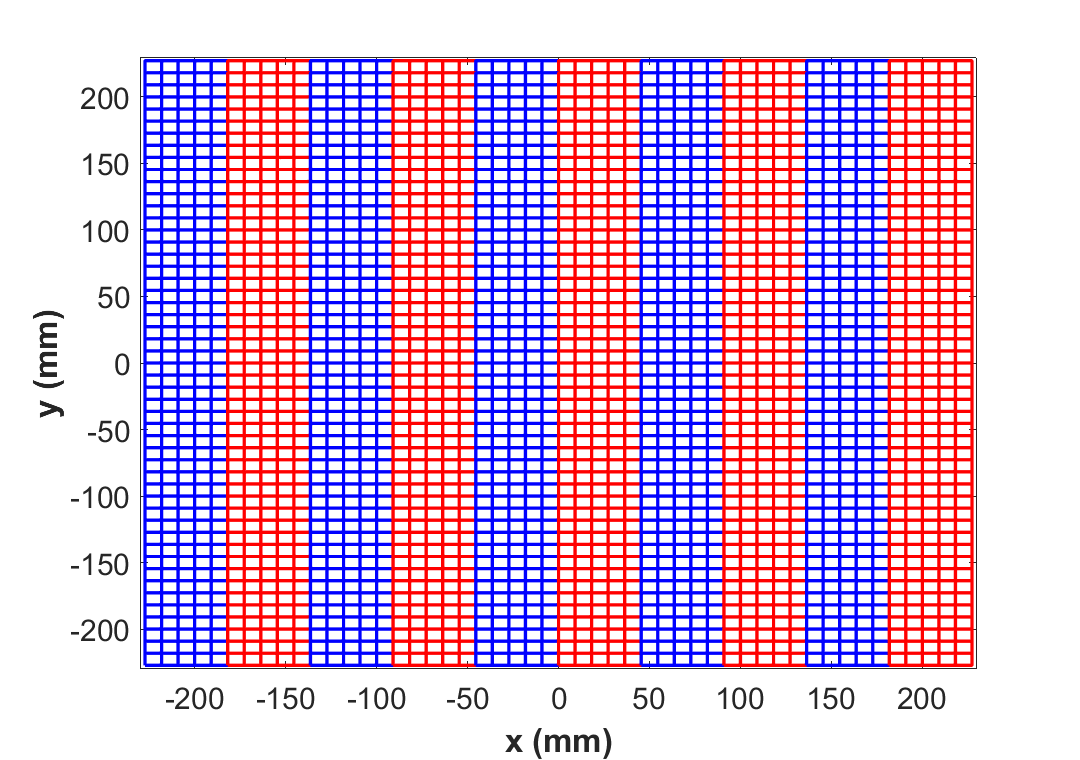
\includegraphics[width=\textwidth]{figures/MeshDiscretization10.png}
  % \caption{A subfigure}
  \label{fig:sub2}
\end{subfigure}
\caption{A figure with two subfigures}
\label{fig:test}
\end{figure}

\section{Direcionamento do Feixe}
Assim, à medida que alteramos o ângulo desejado $θ_s$, a capacidade de controle do feixe é bem comprovada com MoM e modelo de impedância de superfície da teoria da linha de transmissão, como mostrado na Fig. 4. Além disso, podemos notar o efeito correto da faixa invisível e ondas superficiais. Uma vez aumentado o ângulo, observa-se uma modificação maior. Mesmo próximo ao intervalo de meio comprimento de onda, ou seja, $N_ZsL=10$, o nível do lóbulo lateral é afetado.


\begin{figure}[htb]
 \label{RCS5}
    \centering
    \caption{Ilustração da discretização  com a função base pulso} \label{fig_minipage}
    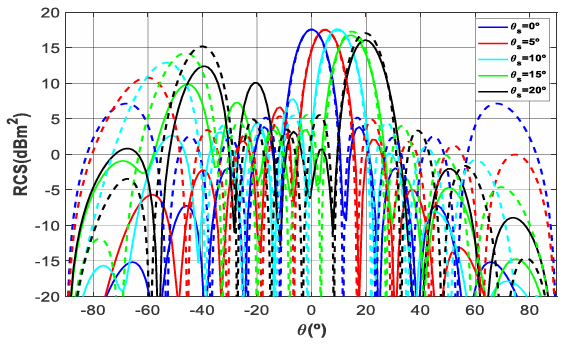
\includegraphics[width=\textwidth]{figures/RCSBeam5.png}
    \legend{Fonte: Produzido pelos autores}
  \hfill
  
\end{figure}


\begin{figure}[htb]
 \label{RCS10}
    \centering
    \caption{Ilustração da discretização  com a função base pulso} \label{fig_minipage}
    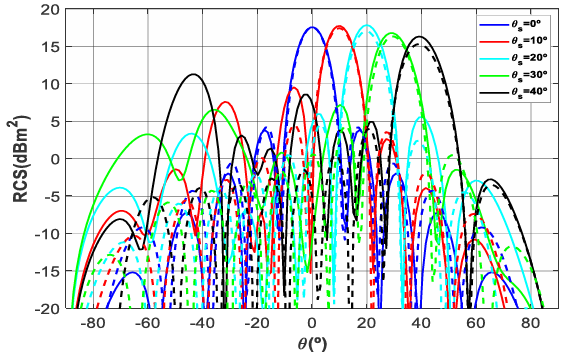
\includegraphics[width=\textwidth]{figures/RCSBeam10.png}
    \legend{Fonte: Produzido pelos autores}
  \hfill
\end{figure}

\section{Direcionamento Ativo}
O comportamento ativo foi testado na Fig. 5 para um ganho de potência de 3dB, ou seja, A=1,5. A forma geral do feixe não muda em comparação com a caixa reflexiva perfeita. Se aplicados outros tipos de coeficientes de matriz, como binomial e Tschebyscheff [11], isso pode levar a um formato de feixe personalizado.
\begin{figure}[htb]
 \label{RCS10Active}
    \centering
    \caption{Ilustração da discretização  com a função base pulso} \label{fig_minipage}
    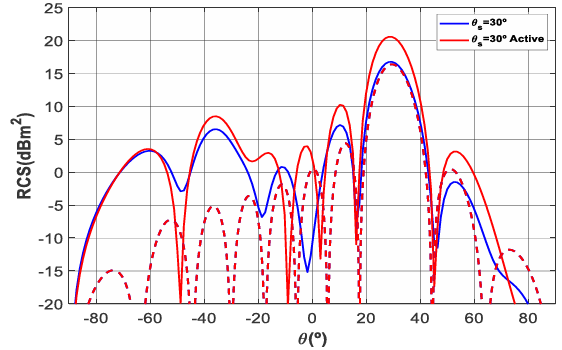
\includegraphics[width=\textwidth]{figures/ActiveRCS10.png}
    \legend{Fonte: Produzido pelos autores}
  \hfill
\end{figure}
% ----------------------------------------------------------
% Finaliza a parte no bookmark do PDF
% para que se inicie o bookmark na raiz
% e adiciona espaço de parte no Sumário
% ----------------------------------------------------------
\phantompart
% ---
% Conclusão
% ---
\chapter{Conclusão}
% ---

\lipsum[31-33]

% ----------------------------------------------------------
% ELEMENTOS PÓS-TEXTUAIS
% ----------------------------------------------------------
\postextual
% ----------------------------------------------------------

% ----------------------------------------------------------
% Referências bibliográficas
% ----------------------------------------------------------
\bibliography{abntex2-MoM-references}

% ----------------------------------------------------------
% Glossário
% ----------------------------------------------------------
%
% Consulte o manual da classe abntex2 para orientações sobre o glossário.
%
%\glossary

% ----------------------------------------------------------
% Apêndices
% ----------------------------------------------------------

% ---
% Inicia os apêndices
% ---
\begin{apendicesenv}

% Imprime uma página indicando o início dos apêndices
%\partapendices

% ----------------------------------------------------------
\chapter{Método de Ondas Planas e Linhas de Transmissão }
% ----------------------------------------------------------

Os elementos da RIS podem ser descritos pelo vetor posição na superfície é dado por

\begin{equation}
    \overline{p}=x\overline{x}+y\overline{y}
\end{equation}
\begin{equation}
\overline{k}_{i}=k_x\overline{a}_x+k_y\overline{a}_y+k_z\overline{a}_z
\end{equation}
\begin{equation}
\overline{k}_{s}=k_x\overline{a}_x+k_y\overline{a}_y-k_z\overline{a}_z
\end{equation}
\begin{equation}
\overline{k}_{i}=k_0(\sin{\theta} \sin{\phi}\overline{a}_x+\sin{\theta}\cos{\phi}\overline{a}_y+\cos{\theta}\overline{a}_z)
\end{equation}
Para incidência de uma onda plana TM , Campos Incidentes,
\begin{subequations}{\label{TMIncFields}}
\begin{equation}
 \overline{E}_{i} =( E_{\theta} \cos{\theta_i}\overline{a}_x -E_{\theta} \sin{\theta_{i}} \overline{a}_z )
 e^{j\kappa (x \sin{\theta} \cos{\phi} + y \sin{\theta} \sin{\phi}+z\cos{\theta})}  
\end{equation}
\begin{equation}
 \overline{H}_{i}=
 \frac{E_{\theta}}{\eta_1} \overline{a}_y
  e^{-jk(\sin{\theta_{i}} x + \cos{\theta_{i}}z) }    
\end{equation}
\end{subequations}
Campos Espalhados, 
\begin{subequations}{\label{TMEsFields}}
\begin{equation}
 \overline{E}_{s}=\Gamma 
 ( E_{\theta}\cos{\theta_{i}} \overline{a}_x 
 +E_{\theta} \sin{\theta_{i}} \overline{a}_z ) 
  e^{-jk(\sin{\theta_{i}} x + \cos{\theta_{i}}z) } 
\end{equation}
\begin{equation}
 \overline{H}_{s}=-\Gamma
 \frac{E_{\theta}}{\eta_1} \overline{a}_y
  e^{-jk(\sin{\theta_{1}} x + \cos{\theta_{1}}z) }    
\end{equation}
\end{subequations}
Campos Transmitidos,
\begin{subequations}{\label{TMTrFields}}
\begin{equation}
 \overline{E}_{tr}= 
 (E^{tr}_{\theta}\cos{\theta_{2}} \overline{a}_x 
 -E^{tr}_{\theta} \sin{\theta_{2}} \overline{a}_z ) 
  e^{-jk(\sin{\theta_{2}} x + \cos{\theta_{2}}z) } 
\end{equation}
\begin{equation}
 \overline{H}_{tr}=
 \frac{E^{tr}_{\theta}}{\eta_2} \overline{a}_y
  e^{-jk(\sin{\theta_{2}} x + \cos{\theta_{2}}z) }    
\end{equation}
\end{subequations}

Considerando 2 meios contínuos com a presença de uma impedância superficial na sua fronteira. Logo pela continuidade dos campos e e do conjunto de equações \ref{BoundaryFields}-\ref{BoundaryCurrent} tem-se, levando em conta que    ${\theta}_{i}={\theta}_{r}$,
\begin{equation}{\label{BoundaryFieldsEiEs}}
(E_1+E_2) \cdot \overline{a}_t=E_{\theta}\cos{\theta_{i}} +
  \Gamma E_{\theta}\cos{\theta_{i}} =E^{tr}_{t}\cos{\theta_{2}}
\end{equation}
\begin{equation}{\label{BoundaryHiHs}}
(H_i+H_s) \cdot \overline{a}_t=[ \frac{E_{\theta}}{\eta_1} -
  \Gamma \frac{E_{\theta} }{\eta_1} ]
\end{equation}

Substituindo \ref{BoundaryFieldsEiEs}-\ref{BoundaryHiHs} em \ref{BoundaryFieldsImp}

\begin{equation}
\cos{\theta_{i}} +
  \Gamma \cos{\theta_{i}} 
  =Z_s 
  [ -\frac{\cos{\theta_{i}}  }{\eta_2\cos{\theta_{2}} } - \frac{\Gamma \cos{\theta_{i}}  }{\eta_2\cos{\theta_{2}} } -
  (-\frac{1}{\eta_1} +\Gamma\frac{1}{\eta_1} )]
\end{equation}
\begin{equation}
\eta_1\cos{\theta_{i}} +
  \Gamma \eta_1\cos{\theta_{i}} 
  =Z_s 
  [ -\frac{\eta_1\cos{\theta_{i}}  }{\eta_2\cos{\theta_{2}} } - \frac{\Gamma \eta_1\cos{\theta_{i}}  }{\eta_2\cos{\theta_{2}} } +1-\Gamma]
\end{equation}
\begin{equation}
\Gamma(\eta_1\cos{\theta_{i}}+\frac{Z_s\eta_1\cos{\theta_{i}}  }{\eta_2\cos{\theta_{2}} }+Z_s)
= 
-\eta_1\cos{\theta_{i}} -\frac{Z_s\eta_1\cos{\theta_{i}}  }{\eta_2\cos{\theta_{2}} }+Z_s
\end{equation}
Assumindo que, $\eta_1^{TM}=\eta_1\cos{\theta_{i}}$ e $\eta_2^{TM}=\eta_2\cos{\theta_{2}}$ e rearranjando as equações
\begin{equation}
\Gamma(1+\frac{{Z_s} }{ \eta_2^{TM}}+\frac{Z_s}{\eta_1^{TM}})
= 
-1 -\frac{Z_s  }{\eta_2^{TM} }+\frac{Z_s}{\eta_1^{TM}}
\end{equation}
\begin{equation}
\Gamma=\frac{-\eta_1^{TM}\eta_2^{TM} -Z_s \eta_1^{TM} +{Z_s}\eta_2^{TM}}
{\eta_1^{TM}\eta_2^{TM}+Z_s \eta_1^{TM} +{Z_s}\eta_2^{TM}}
\end{equation}

\begin{equation}
\Gamma=\frac{-\eta_1^{TM}(\eta_2^{TM}+Z_s) +Z_s \eta_2^{TM} }
{\eta_1^{TM}(\eta_2^{TM}+Z_s) +Z_s \eta_2^{TM}}
\end{equation}

Dividindo por $(\eta_2^{TM}+Z_s) $

\begin{equation}{\label{CoefReflexaoParaleloZsEta2}}
   \Gamma= \frac{\frac{Z_s \eta_2^{TM} }{\eta_2^{TM}+Z_s}-\eta_1^{TM}}
    {\frac{Z_s \eta_2^{TM} }{\eta_2^{TM}+Z_s}+\eta_1^{TM}}
\end{equation}

Se olharmos pelo ponto de vista de linhas de transmissão, o coeficiente de reflexão  é calculado em relação a impedância intrínseca do meio 1 e a impedância de entrada vista na superfície ou impedância de entrada, o circuito paralelo  entre $Z_s$ e a impedância intrínseca da onda incidente $\eta^{TM}_{2}$. Logo a impedância vista da RIS representada pela impedância superficial e o meio 2 que pode ser considerada uma linha de transmissão, é dada por,

\begin{equation}{\label{ImpedanciaZinParaleloZsEta2}}
   Z_{in}= \frac{Z_s \eta_2^{TM} }{\eta_2^{TM}+Z_s}
\end{equation}
Se o meio 2 é o idêntico ao meio 1, e todos os dois, o espaço Livre, o caso da RIS, pois a impedância superficial encapsula toda estrutura, temos $\eta^{TM}_{2}=\eta^{TM}_1=\eta^{TM}_0$

E o coeficiente de reflexão se deduz como,
\begin{equation}
   \Gamma= \frac{Z_{in}-\eta_1^{TM}}
    {Z_{in}+\eta_1^{TM}}
\end{equation}
Se os dois meios forem o espaço livre,
\begin{equation}
    \Gamma=\frac{-\eta_0}{2Z_s+\eta_0}
\end{equation}
A impedância superficial em relação ao coeficiente de reflexão

% ----------------------------------------------------------
\chapter{MoMCSL}
% ----------------------------------------------------------
\subsection{ Representação Numérica}
O MoM  bidimensional por [Costa]resolve o prolema completamente considerando-o como um sistema linear discreto, por ser um método numérico.  A solução do sistema é a corrente de excitação, dada pela constantes complexas não conhecidas $J_{x,y}^{n,m} \ $ .Logo, a densidade de corrente pode ser expandida em termos de uma função base, que no caso, é a função pulso retangular com dimensão , de acordo com os procedimentos do MoM bidimensional. A escolha por essa base, no meu entendimento, se dá por ser mais simples a implementação numérica, ter uma alta acurácia, além de ser conforme com as seções retangulares que encapsulam as características de cada elemento da IRS. Então se discretizarmos a superfície $S$  com comprimento $L$  e largura $W$, de acordo com a ilustração da Fig. \ref{DiscretizaçãoXY}, com $N_x-1$ colunas e $N_y$ linhas de tensão para a excitação $J_x$, e $N_x$ colunas e $N_y-1$ linhas de tensão para a excitação $J_y$, igualmente espaçadas $\Delta l_x$  em $x$ e $\Delta l_y$ em $y$.  Logo, tem-se,
\begin{subequations}
    \begin{equation}
    L=N_x {\Delta l}_x
\end{equation}
  \begin{equation}
    W=N_y {\Delta l}_y
\end{equation}
\end{subequations}
A densidade de corrente pode ser escrita como,
\begin{equation}{\label{ExpansãoJx}}
    \overline{J}(\overline{p}) \cdot \overline{a}_x=J_x(n,m)=\sum_{m=1}^{N_x-1}\sum_{n=1}^{N_y} J_{x}^{n,m}P_{J_x}^{n,m}(\overline{p})
\end{equation}
\begin{equation}{\label{ExpansãoJy}}
    \overline{J}(\overline{p}) \cdot \overline{a}_y=J_y(n,m)=
\sum_{m=1}^{N_x}\sum_{n=1}^{N_y-1} J_{y}^{n,m}P_{J_y}^{n,m} (\overline{p})   
\end{equation}

\begin{figure}[htb]
 \label{DiscretizaçãoXY}


    \centering
    \caption{Ilustração da discretização  com a função base pulso} \label{fig_minipage}
    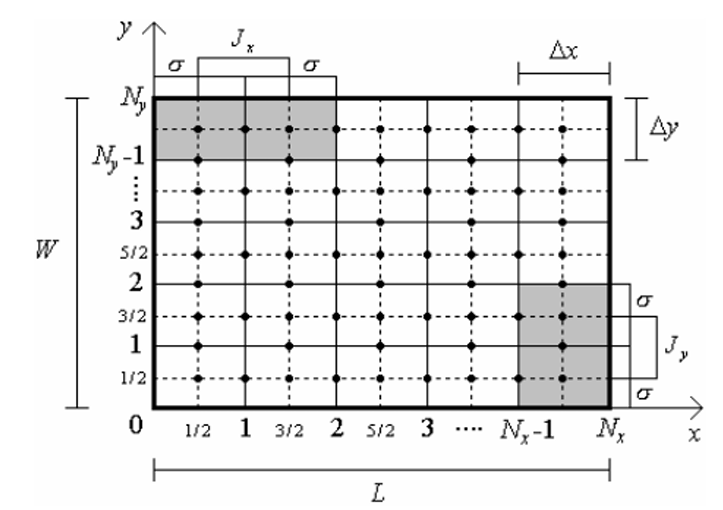
\includegraphics[width=\textwidth]{figures/MalhaDiscretizacao.png}
    \legend{Fonte: Produzido pelos autores}
  \hfill

\end{figure}
Sendo $N_x$, o número de discretizações em $x$, $N_y$ o número de discretizações em y, e as condições de contorno da função pulso,
\begin{equation}
     P_{J_x}^{n,m}(\overline{p})=  
     \begin{cases}
      1 \ \ x_{n,m}^{-} \leq x < x_{n,m}^{+},\ y_{(n-1),m} \leq y < y_{n}\\
      0 \ \ fora \ do \ limite \\
    \end{cases}  
\end{equation}
\begin{equation}
     P_{J_y}^{n,m}(\overline{p})=  
     \begin{cases}
      1 \ \  x_{n,(m-1)} \leq x < x_{n,m}, \ y_{n,m}^{-} \leq y < y_{n,m}^{+} \\
      0 \ \ fora \ do \ limite \\
    \end{cases}  
\end{equation}
As disposição das correntes e da função pulso retangular impõem a condição de contorno ao problema, de que as correntes normais nas bordas devem se anular, e que existam sim, densidades de corrente tangenciais a borda. Assim como assegura que as cargas que originam e/ou terminam, tanto a densidade de corrente em $J_x$, quanto a densidade corrente em $J_y$ se sobreponham, respeitando as equações de Maxwell no domínio numérico tanto para rotação do campos como para divergência. Um exemplo da borda inferior esquerda com os vetores posições e distância está ilustrada na Fig. \ref{PulsosVetorPosicaoIlustracao} . A função de teste é escolhida de maneira que porta as características da discretização espacial para o caminho de integração da diferença de potencial em $x$ ou em $y$.  Para a integração em $x$ temos
 \begin{equation}{\label{FunçaoTesteJx}}
     w_{m}(\overline{p})= P_{J_x}^{n,m}(\overline{p})\delta(\overline{p}-\overline{p}^{{m,n}}_{J^{-}_y})\overline{a}_x =
       \begin{cases}
      1, \ \ x_{n,m}^{-} \leq x < x_{n,m}^{+},\ \ y=y_{n,m}^{-}\\
      0, \ \ fora \ do \ limite \\
    \end{cases}  
 \end{equation}
Sendo que e  $x^{+}_{n,m}=\frac{x_{n,m+1}-x_{n,m}}{2}$Enquanto para a integração em $y$
\begin{equation}{\label{FunçaoTesteJx}}
     w_{m}(\overline{p})= P_{J_y}^{n,m}(\overline{p})\delta(\overline{p}-\overline{p}^{{m,n}}_{J^{-}_x})\overline{a}_y =
       \begin{cases}
      1 \ \ x=x_{n,m}^{-}, \ \ y_{n,m}^{-} \leq y < y_{n,m}^{+}  \\
      0 \ \ fora \ do \ limite \\
    \end{cases}  
 \end{equation}
sendo que as coordenadas discretas são definidas, 
 \begin{subequations}
    \begin{equation}
    x_{n,m}=m{\Delta l}_x
\end{equation}
    \begin{equation}
    x^{-}_{n,m}=x_{n,m}-\frac{{\Delta l}_x}{2}
\end{equation}
  \begin{equation}
    x^{+}_{n,m}=x_{n,m}+\frac{{\Delta l}_x}{2}
\end{equation}
      \begin{equation}
    y_{n,m}=n{\Delta l}_y
\end{equation}
  \begin{equation}
    y^{-}_{n,m}=y_{n,m}-\frac{{\Delta l}_y}{2}
\end{equation}
  \begin{equation}
    y^{+}_{n,m}=y_{n,m}+\frac{{\Delta l}_y}{2}
\end{equation}
\end{subequations}

\begin{figure}[htb]
 \label{PulsosVetorPosicaoIlustracao}
 \centering
  \begin{minipage}{\textwidth}
    \centering
    \caption{Exemplo da Discretização com o Vetor Posição da Função Pulso} \label{fig_minipage_imagem2}
    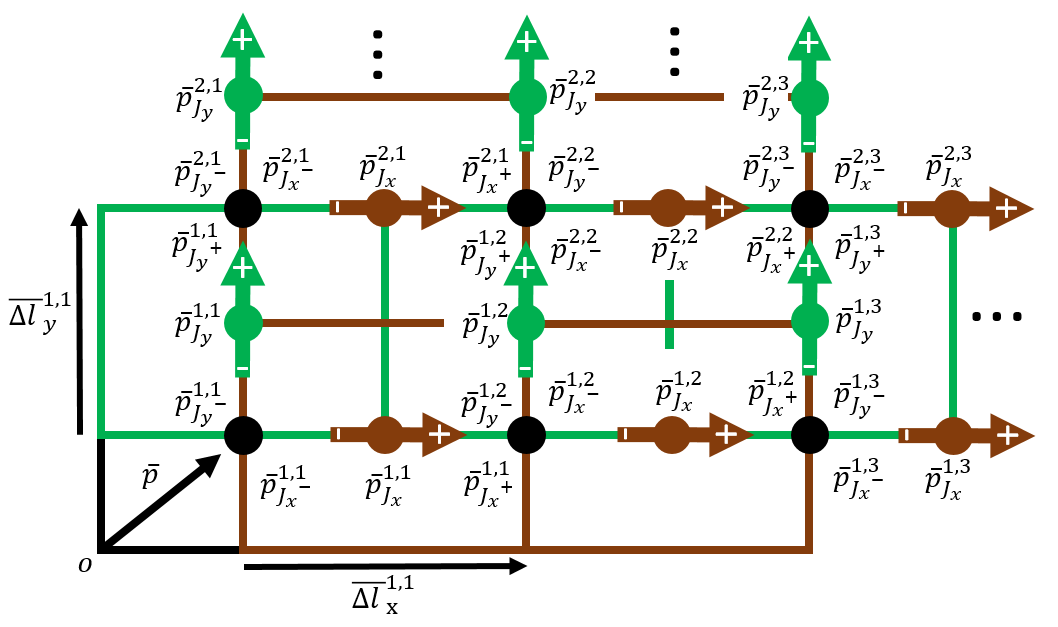
\includegraphics[width=14cm, height=8.5cm]{figures/PulsosVetorPosicaoIlustracao.png}
    \legend{Fonte: Produzido pelos autores}
  \end{minipage}
  \hfill

\end{figure}
Portanto, ao efetuar  a integração com a função teste, transforma-se parcialmente a continuidade do problema para o domínio numérico. Aproximando a continuidade da superfície, sem desconsiderar a interação dos elementos. A tensão em cada elemento em $x$ pode ser escrita, substituindo as expansões da densidade de corrent \ref{ExpansãoJx} -\ref{ExpansãoJy} e a função de teste \ref{ FunçaoTesteJx} em \ref{ProdutoInternoMoM}
\begin{equation}{\label{ProdutoInternoMoMDiscreto}}
\begin{aligned}
 \Delta V_{x}^{n,m}=Z_s^{n,m}    \int \limits_{x_{n,m}^{-}}^{x_{n,m}^{+}} (J_{x}^{n,m} P_{J_x}^{n,m}(\overline{p}) \delta (\overline{p}-\overline{p}^{{mn}}_{J^{-}_y}))dx \\
      +
 \int \limits_{x_{n,m}^{-}}^{x_{n,m}^{+}}    j\omega \mu  \iint\limits_{S} J_x(\overline{p^{'}}) P_{J_x}^{n,m}(\overline{p})\delta (\overline{p}-\overline{p}^{{mn}}_{J^{-}_y}) ) \frac{e^{-j k R}}{4 \pi R} dS^{'}   dx
 \\
  -  \int \limits_{x_{n,m}^{-}}^{x_{n,m}^{+}}     \frac{\partial }{\partial x}\biggl[ \frac{1}{j\omega \epsilon}\iint\limits_S  (\sum_{n^{'}=1}^{N_x-1}\sum_{m^{'}=1}^{N_y}\frac{\partial (J_{x}^{n^{'},m^{'}}P_{J_x}^{n^{'},m^{'}}(\overline{p^{'}})  )}{\partial x}  )P_{J_x}^{n,m}(\overline{p})\delta (\overline{p}-\overline{p}^{{mn}}_{J^{-}_y})) \frac{e^{-j k R}}{4 \pi R} dS^{'}  \biggl] dx \\
    -  \int \limits_{x_{n,m}^{-}}^{x_{n,m}^{+}}     \frac{\partial }{\partial x}\biggl[ \frac{1}{j\omega \epsilon}\iint\limits_S  (\sum_{n^{'}=1}^{N_x}\sum_{m^{'}=1}^{N_y-1} \frac{\partial (J_{y}^{n^{'},m^{'}}P_{J_y}^{n^{'},m^{'}} (\overline{p^{'}})    )}{\partial y}  )P_{J_x}^{n,m}(\overline{p})\delta (\overline{p}-\overline{p}^{{mn}}_{J^{-}_y})) \frac{e^{-j k R}}{4 \pi R} dS^{'}  \biggl] dx

\end{aligned}
\end{equation}
Onde,  

\begin{equation}
     \Delta V_{x}^{n,m}=\int \limits_{\overline{\Delta l}_x}E_{x} \cdot w_m dx
\end{equation}
Usando integração numérica do ponto médio na integral do produto interno com a função de teste,  tem-se,
\begin{equation}
\begin{aligned}
      \Delta V_{x}^{n,m}= Z_s^{n,m}  J_{x}^{n,m}  {\Delta l}_x
      +
j\omega \mu   {\Delta l}^{{'}}_x \sum_{m^{'}=1}^{N_x-1}\sum_{n^{'}=1}^{N_y} J_{x}^{n^{'},m^{'}} \iint\limits_{S}  P_{J_x}^{n^{'},m^{'}}(\overline{p^{'}})   \frac{e^{-j k |\overline{p}_{{J_x}}^{n,m}-\overline{p^{'}}|}}{4 \pi |\overline{p}_{{J_x}}^{n,m}-\overline{p^{'}}|} dS^{'}    \\
   + 
   \frac{1}{j\omega \epsilon}\biggl[ \iint\limits_{S} \sum_{n^{'}=1}^{N_x-1}\sum_{m^{'}=1}^{N_y}\frac{\partial (J_{x}^{n^{'},m^{'}}P_{J_x}^{n^{'},m^{'}}(\overline{p^{'}})  )}{\partial x}  \frac{e^{-j k R}}{4 \pi R} dS^{'}  \biggl] \biggl |_{\overline{p}_{{J_x^{+}}}^{n,m}}^{\overline{p}_{{J_x^{-}}}^{n,m}}\\
  + 
  \frac{1}{j\omega \epsilon}\biggl[ \iint\limits_{S}\sum_{n^{'}=1}^{N_x}\sum_{m^{'}=1}^{N_y-1} \frac{\partial (J_{y}^{n^{'},m^{'}}P_{J_y}^{n^{'},m^{'}} (\overline{p^{'}})    )}{\partial y}  \frac{e^{-j k R}}{4 \pi R} dS^{'}  \biggl] \biggl |_{\overline{p}_{{J_x^{+}}}^{n,m}}^{\overline{p}_{{J_x^{-}}}^{n,m}}
\end{aligned}
\end{equation}
Expandindo mais a equação,
\begin{equation}
\begin{aligned}
      \Delta V_i^{n,m}=Z_s^{n,m}  J_{x}^{n,m} {\Delta l}_x
      +
j\omega \mu  {\Delta l}^{{'}}_x \sum_{m^{'}=1}^{N_x-1}\sum_{n^{'}=1}^{N_y} J_{x}^{n^{'},m^{'}} \iint\limits_{S}  P_{J_x}^{n^{'},m^{'}}(\overline{p^{'}})   \frac{e^{-j k |\overline{p}_{{J_x}}^{n,m}-\overline{p^{'}}|}}{4 \pi |\overline{p}_{{J_x}}^{n,m}-\overline{p^{'}}|} dS^{'}    \\
+
    \frac{1}{j\omega \epsilon}\biggl[\sum_{m^{'}=1}^{N_x-1}\sum_{n^{'}=1}^{N_y} J_{x}^{n^{'},m^{'}} \iint\limits_{S}  \frac{\partial (P_{J_x}^{n^{'},m^{'}}(\overline{p^{'}})    )}{\partial x}  \frac{e^{-j k |\overline{p}_{{J_x^{-}}}^{n,m}-\overline{p^{'}}|}}{4 \pi |\overline{p}_{{J_x^{-}}}^{n,m}-\overline{p^{'}}|} dS^{'}  \biggl] \\
    -
      \frac{1}{j\omega \epsilon}\biggl[ \sum_{m^{'}=1}^{N_x-1}\sum_{n^{'}=1}^{N_y} J_{x}^{n^{'},m^{'}} \iint\limits_{S}  \frac{\partial (P_{J_x}^{n^{'},m^{'}}(\overline{p^{'}})    )}{\partial x} \frac{e^{-j k |\overline{p}_{{J_x^{+}}}^{n,m}-\overline{p^{'}}|}}{4 \pi |\overline{p}_{{J_x^{+}}}^{n,m}-\overline{p^{'}}|}dS^{'}  \biggl] \\
  +    
       \frac{1}{j\omega \epsilon}\biggl[\sum_{m^{'}=1}^{N_x}\sum_{n^{'}=1}^{N_y-1} J_{y}^{n^{'},m^{'}} \iint\limits_{S}  \frac{\partial (P_{J_y}^{n^{'},m^{'}}(\overline{p^{'}})    )}{\partial y}  \frac{e^{-j k |\overline{p}_{{J_x^{-}}}^{n,m}-\overline{p^{'}}|}}{4 \pi |\overline{p}_{{J_x^{-}}}^{n,m}-\overline{p^{'}}|} dS^{'}  \biggl] \\
    -
      \frac{1}{j\omega \epsilon}\biggl[ \sum_{m^{'}=1}^{N_x}\sum_{n^{'}=1}^{N_y-1} J_{y}^{n^{'},m^{'}} \iint\limits_{S}  \frac{\partial (P_{J_y}^{n^{'},m^{'}}(\overline{p^{'}})    )}{\partial y} \frac{e^{-j k |\overline{p}_{{J_x^{+}}}^{n,m}-\overline{p^{'}}|}}{4 \pi |\overline{p}_{{J_x^{+}}}^{n,m}-\overline{p^{'}}|}dS^{'}  \biggl] \\
\end{aligned}
\end{equation}
Aplicando a derivada da função pulso, e definindo a condição de contorno das áreas de integração das cargas discretas de acordo com a Fig. \ref{CargasDeltaSIlustracao},
\begin{figure}[htb]
 \label{CargasDeltaSIlustracao}
 \centering
  \begin{minipage}{\textwidth}
    \centering
    \caption{Área de integração das Cargas do Potencial Escalar} \label{fig_minipage_imagem2}
    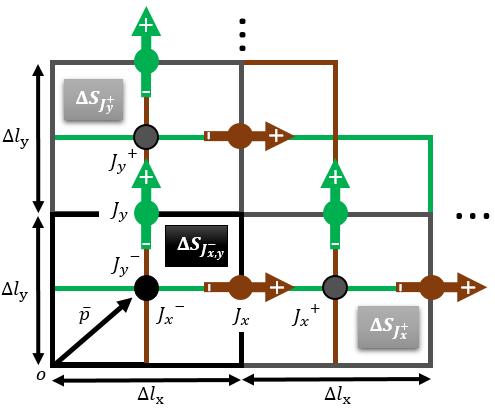
\includegraphics[width=10cm]{figures/CargasDeltaSIlustracao.png}
    \legend{Fonte: Produzido pelos autores}
  \end{minipage}
  \hfill

\end{figure}
\begin{equation}\label{DVnmPotencialScalarPulse2Delta}
\begin{aligned}
      \Delta V_i^{n,m}=Z_s^{n,m}  J_{x}^{n,m} {\Delta l}_x
      +
    j\omega \mu   {\Delta l}^{{'}}_x \sum_{m^{'}=1}^{N_x-1}\sum_{n^{'}=1}^{N_y} J_{x}^{n^{'},m^{'}} \iint\limits_{S}  P_{J_x}^{n^{'},m^{'}}(\overline{p^{'}})   \frac{e^{-j k |\overline{p}_{{J_x}}^{n,m}-\overline{p^{'}}|}}{4 \pi |\overline{p}_{{J_x}}^{n,m}-\overline{p^{'}}|} dS^{'}    \\ \\
    +
    \frac{1}{j\omega \epsilon}\biggl[ \sum_{n=1}^{N_x-1}\sum_{m=1}^{N_y}J_{x}^{n^{'},m^{'}} 
\biggl(\iint \limits_{{\Delta S}^{'}_{J_x^-}}  \frac{ \delta(\overline{p^{'}}-\overline{p}^{n^{'},m^{'}}_{J_x^{-}})}{\Delta l^{'}_x } 
- \iint \limits_{{\Delta S}^{'}_{J_x^{+}}}  \frac{ \delta(\overline{p^{'}}-\overline{p}^{n^{'},m^{'}}_{J_x^{+}})}{\Delta l^{'}_x } 
\biggl)
\frac{e^{-j k |\overline{p}_{{J_x^{-}}}^{n,m}-\overline{p^{'}}|}}{4 \pi |\overline{p}_{{J_x^{-}}}^{n,m}-\overline{p^{'}}|} dS^{'}  \biggl] \\
    -
      \frac{1}{j\omega \epsilon}\biggl[ \sum_{n=1}^{N_x-1}\sum_{m=1}^{N_y}J_{x}^{n^{'},m^{'}} 
\biggl(\iint \limits_{{\Delta S}^{'}_{J_x^-}}  \frac{ \delta(\overline{p^{'}}-\overline{p}^{n^{'},m^{'}}_{J_x^{-}})}{\Delta l^{'}_x } 
- \iint \limits_{{\Delta S}^{'}_{J_x^{+}}}  \frac{ \delta(\overline{p^{'}}-\overline{p}^{n^{'},m^{'}}_{J_x^{+}})}{\Delta l^{'}_x } 
\biggl)
\frac{e^{-j k |\overline{p}_{{J_x^{+}}}^{n,m}-\overline{p^{'}}|}}{4 \pi |\overline{p}_{{J_x^{+}}}^{n,m}-\overline{p^{'}}|}dS^{'}  \biggl] \\
    +
    \frac{1}{j\omega \epsilon}\biggl[ \sum_{n=1}^{N_x}\sum_{m=1}^{N_y-1}J_{y}^{n^{'},m^{'}} 
\biggl(\iint \limits_{{\Delta S}^{'}_{J_y^-}}  \frac{ \delta(\overline{p^{'}}-\overline{p}^{n^{'},m^{'}}_{J_y^{-}})}{\Delta l^{'}_y } 
- \iint \limits_{{\Delta S}^{'}_{J_y^{+}}}  \frac{ \delta(\overline{p^{'}}-\overline{p}^{n^{'},m^{'}}_{J_y^{+}})}{\Delta l^{'}_y } 
\biggl)
\frac{e^{-j k |\overline{p}_{{J_x^{-}}}^{n,m}-\overline{p^{'}}|}}{4 \pi |\overline{p}_{{J_x^{-}}}^{n,m}-\overline{p^{'}}|} dS^{'}  \biggl] \\
    -
      \frac{1}{j\omega \epsilon}\biggl[ \sum_{n=1}^{N_x}\sum_{m=1}^{N_y-1}J_{y}^{n^{'},m^{'}} 
\biggl(\iint \limits_{{\Delta S}^{'}_{J_y^-}}  \frac{ \delta(\overline{p^{'}}-\overline{p}^{n^{'},m^{'}}_{J_y^{-}})}{\Delta l^{'}_y } 
- \iint \limits_{{\Delta S}^{'}_{J_y^{+}}}  \frac{ \delta(\overline{p^{'}}-\overline{p}^{n^{'},m^{'}}_{J_y^{+}})}{\Delta l^{'}_y } 
\biggl)\frac{e^{-j k |\overline{p}_{{J_x^{+}}}^{n,m}-\overline{p^{'}}|}}{4 \pi |\overline{p}_{{J_x^{+}}}^{n,m}-\overline{p^{'}}|}dS^{'}  \biggl] \\
\end{aligned}
\end{equation}
Uma vez que podemos escrever as integrais do potencial escalar como,
\begin{subequations}
\begin{equation}
    \Phi_{xx}(n^{'},m^{'},n,m)=\iint\limits_{{\Delta S}^{'}}   P_{J_x}^{n^{'},m^{'}}(\overline{p^{'}})   \frac{e^{-j k |\overline{p}_{{J_x}}^{n,m}-\overline{p^{'}}|}}{4 \pi |\overline{p}_{{J_x}}^{n,m}-\overline{p^{'}}|} dS^{'}  =
 \iint\limits_{{\Delta S}^{'}}  \frac{e^{-j k |\overline{p}_{{J_x}}^{n,m}-\overline{p}_{{J_x}}^{n^{'},m^{'}}|}}{4 \pi |\overline{p}_{{J_x}}^{n,m}-\overline{p}_{{J_x}}^{n^{'},m^{'}}|} dS^{'}
\end{equation}
\begin{equation}
    \Phi_{xx}^{--}(n^{'},m^{'},n,m)=\iint\limits_{{\Delta S}^{'}_{J_x^{-}}}    \frac{ \delta(\overline{p^{'}}-\overline{p}^{n^{'},m^{'}}_{J_x^{-}})}{{\Delta l}_x^{'} } \frac{e^{-j k |\overline{p}_{{J_x^{-}}}^{n,m}-\overline{p^{'}}|}}{4 \pi |\overline{p}_{{J_x^{-}}}^{n,m}-\overline{p^{'}}|} dS^{'}  =
\iint\limits_{{\Delta S}^{'}_{J_x^{-}}}  
\frac{e^{-j k |\overline{p}_{J_{x}^{-}}^{n,m}-\overline{p}_{J_{x}^{-}}^{n^{'},m^{'}}|}}{4 \pi {\Delta l}_x^{'} |\overline{p}_{J_{x}^{-}}^{n,m}-\overline{p}_{J_{x}^{-}}^{n^{'},m^{'}}|} dS^{'}
\end{equation}
\begin{equation}
    \Phi_{xx}^{+-}(n^{'},m^{'},n,m)=\iint\limits_{{\Delta S}^{'}_{J_x^{+}}}    \frac{ \delta(\overline{p^{'}}-\overline{p}^{n^{'},m^{'}}_{J_x^{+}})}{{\Delta l}_x^{'} } \frac{e^{-j k |\overline{p}_{{J_x^{-}}}^{n,m}-\overline{p^{'}}|}}{4 \pi |\overline{p}_{{J_x^{-}}}^{n,m}-\overline{p^{'}}|} dS^{'}  =
  \iint\limits_{{\Delta S}^{'}_{J_x^{+}}}    \frac{e^{-j k |\overline{p}_{J_{x}^{-}}^{n,m}-\overline{p}_{J_{x}^{+}}^{n^{'},m^{'}}|}}{4 \pi {\Delta l}_x^{'}|\overline{p}_{J_{x}^{-}}^{n,m}-\overline{p}_{J_{x}^{+}}^{n^{'},m^{'}}|} dS^{'}
\end{equation}
\begin{equation}
    \Phi_{xx}^{-+}(n^{'},m^{'},n,m)=\iint\limits_{{\Delta S}^{'}_{J_x^{-}}}    \frac{ \delta(\overline{p^{'}}-\overline{p}^{n^{'},m^{'}}_{J_x^{-}})}{{\Delta l}_x^{'} } \frac{e^{-j k |\overline{p}_{{J_x^{+}}}^{n,m}-\overline{p^{'}}|}}{4 \pi |\overline{p}_{{J_x^{+}}}^{n,m}-\overline{p^{'}}|} dS^{'}  =
  \iint\limits_{{\Delta S}^{'}_{J_x^{-}}}  \frac{e^{-j k |\overline{p}_{J_{x}^{+}}^{n,m}-\overline{p}_{J_{x}^{-}}^{n^{'},m^{'}}|}}{4 \pi {\Delta l}_x^{'} |\overline{p}_{J_{x}^{+}}^{n,m}-\overline{p}_{J_{x}^{-}}^{n^{'},m^{'}}|} dS^{'}
\end{equation}
\begin{equation}
    \Phi_{xx}^{++}(n^{'},m^{'},n,m)=\iint\limits_{{\Delta S}^{'}_{J_x^{+}}}     \frac{ \delta(\overline{p^{'}}-\overline{p}^{n^{'},m^{'}}_{J_x^{+}})}{{\Delta l}_x^{'} } \frac{e^{-j k |\overline{p}_{{J_x^{+}}}^{n,m}-\overline{p^{'}}|}}{4 \pi |\overline{p}_{{J_x^{+}}}^{n,m}-\overline{p^{'}}|} dS^{'}  =
 \iint\limits_{{\Delta S}^{'}_{J_x^{+}}}    \frac{e^{-j k |\overline{p}_{J_{x}^{+}}^{n,m}-\overline{p}_{J_{x}^{+}}^{n^{'},m^{'}}|}}{4 \pi {\Delta l}_x^{'} |\overline{p}_{J_{x}^{+}}^{n,m}-\overline{p}_{J_{x}^{+}}^{n^{'},m^{'}}|} dS^{'}
\end{equation}
\end{subequations}
Analogamente para as partes contendo as soluções das correntes em y.
Entende-se fisicamente que a função $\delta$ representaria a presença e posição da densidade de cargas discretas negativas e positvas que originam e terminam, tanto as densidade de corrente discretas $J_x$ como as  densidades de correntes discretas $J_y$. Reorganizando a equação \ref{DVnmPotencialScalarPulse2Delta}

\begin{equation}\label{TensãoCadaElementoNM}
\begin{aligned}
    \Delta V_{x}^{n,m}=Z_s^{n,m}  J_{x}^{n,m} \Delta l_x 
    + 
    j\omega \mu  \Delta l_x \sum^{N_y}_{n^{'}=1} \sum^{N_x -1}_{m^{'}=1} \Phi_{xx}(n^{'},m^{'},n,m) \\  
    +
    \frac{1}{j \omega \epsilon} \sum^{N_y}_{n^{'}=1} \sum^{N_x -1}_{m^{'}=1}(\Phi_{xx}^{++}(n^{'},m^{'},n,m)-\Phi_{xx}^{+-}(n^{'},m^{'},n,m)-\Phi_{xx}^{-+}(n^{'},m^{'},n,m)+\Phi_{xx}^{--}(n^{'},m^{'},n,m)) \\
    +
    \frac{1}{j \omega \epsilon} \sum^{N_y-1}_{n^{'}=1} \sum^{N_x}_{m^{'}=1}(\Phi_{xy}^{++}(n^{'},m^{'},n,m)-\Phi_{xy}^{+-}(n^{'},m^{'},n,m)-\Phi_{xy}^{-+}(n^{'},m^{'},n,m)+\Phi_{xy}^{--}(n^{'},m^{'},n,m))
\end{aligned}
\end{equation}
Onde os termos com exponente $xx$ referem ao efeito da convolução entre elementos de densidade de carga ou corrente $x$ em $x$,  os termos com exponente $xy$, o efeito da convolução dos elementos de densidade de carga em ou corrente $y$ em $x$ . Seguindo procedimento analogo, a tensão $\Delta V_y$ pode ser encontrada. 
\subsection{Representação Matricial}
Os índices $n,m$ referentes, respectivamente, as linhas e colunas da discretização, tanto para a densidade de corrente em $x$ quanto em $y$, serão transformados em um índice único $I$ ou $J$.  No caso o $J$ se refere ao elemento analisado, e $I$ referente a contribuição dos outros elementos.

\begin{equation}
\begin{cases}
I,J=(n-1) N_x+m ,\ sendo \ J_x^{nm}=J_{J} \ ou \ J_{I}\\
I,J=N_y(N_x-1)+(n-1) N_x+m ,\ sendo \ J_y^{nm}=J_{J} \ ou \ J_{I}
\end{cases}
\end{equation}
Os termos com somatórios, representam o campo espalhado, que em sua essência possui a convolução da função de green com os outros elementos de corrente em $x$ e/ou $y$,  representados como $Z_{JI}$. Logo, a tensão no elemento $J$ em função dos outros elementos, pode ser expressa como a seguir,

\begin{equation}
    {\Delta V}_J=Z^J_s J_I \Delta l_J-  \sum^{N_t}_{I=1}  Z_{JI}J_I
\end{equation}
Um obstáculo para essa formulação é que o potencial magnético em $x$ não depende da corrente em $y$ e, vice-versa. Para remediar, utiliza-se um produto escalar do vetor comprimento  $\overline{\Delta l}_J$  do elemento de densidade de corrente $J$ com o vetor comprimento $\overline{\Delta l}_I$ do elemento de densidade de corrente $I$, para assim, anular o efeito da componente ortogonal . Portanto, temos,
\begin{equation}
   Z_{JI}=-   
j\omega \mu  \overline{\Delta l}_J \cdot \overline{\Delta l}_I  \Phi_{JI}\\ 
 -
    \frac{1}{j \omega \epsilon}  (\Phi_{JI}^{++}-\Phi_{JI}^{+-}-\Phi_{JI}^{-+}+\Phi_{JI}^{--}) \\
\end{equation}
Já as equações do potencial escalar são similares, tanto para a $J_x$ quanto para $J_y$, dependentes apenas do vetor posição positivo ou negativo das cargas. Logo, generaliza-se a convolução do vetor magnético e do potêncial escalar para os elementos $JI$
\begin{subequations}
\begin{equation}
\Phi_{JI} =\frac{1}{j\omega \epsilon {\Delta l}_I}\iint\limits_{{\Delta S}^{'}}  \frac{e^{-j k R_{JI}}}{4 \pi R_{JI}} dS^{'} \Biggl |_{P_{J_{J}}}^{P_{J_{I}}}
\end{equation}
\begin{equation}
  \Phi_{JI}^{++} =\frac{1}{j\omega \epsilon {\Delta l}_I}\iint\limits_{{\Delta S}^{'}}  \frac{e^{-j k R_{JI}^{++}}}{4 \pi R_{JI}^{++}} dS^{'} \Biggl |_{P_{J_{I}^{+}}}^{P_{J_{J}^{+}}}
  \end{equation}
\begin{equation}
  \Phi_{JI}^{+-} =\frac{1}{j\omega \epsilon {\Delta l}_I}\iint\limits_{{\Delta S}^{'}}   \frac{e^{-j k R_{JI}^{+-}}}{4 \pi R_{JI}^{+-}} dS^{'} \Biggl |_{P_{J_{I}^{+}}}^{P_{J_{J}^{-}}}
  \end{equation}
  \begin{equation}
  \Phi_{JI}^{-+} =\frac{1}{j\omega \epsilon {\Delta l}_I}\iint\limits_{{\Delta S}^{'}}   \frac{e^{-j k R_{JI}^{-+}}}{4 \pi R_{JI}^{-+}} dS^{'}\Biggl |_{P_{J_{I}^{-}}}^{P_{J_{J}^{+}}}
  \end{equation}
   \begin{equation}
  \Phi_{JI}^{--} =\frac{1}{j\omega \epsilon {\Delta l}_I}\iint\limits_{{\Delta S}^{'}}   \frac{e^{-j k R_{JI}^{--}}}{4 \pi R_{JI}^{--}} dS^{'} \Biggl |_{P_{J_{J}^{-}}}^{P_{J_{I}^{-}}}
  \end{equation}

\end{subequations}
Os pontos ($+$$ ou $$-$) significam o vetor posição das cargas negativas e positivas do elemento de densidade de corrente $I$ ou $J$, e $R_{JI}$ a distâncias entre elas. As integrais  são aproximadas numericamente para $kR<<1$

\begin{equation}
   \Phi= \begin{cases}
        \frac{1}{4 \pi \Delta l} \biggl[\Delta l \times \ln{\frac{(\sqrt{{\Delta l}^2+\Delta^2}+\Delta)}{(\sqrt{{\Delta l}^2+\Delta^2}-\Delta)}} 
        + \Delta  \times \ln{\frac{(\sqrt{{\Delta l}^2+\Delta^2}+\Delta)}{(\sqrt{{\Delta l}^2+\Delta^2}-\Delta)}} -jk\Delta l \times \Delta
        \biggl], \ I=J \\
     \frac{1}{4 \pi \Delta l} \frac{e^{-jkR}}{R} ( \Delta l \times \Delta), I \neq J
    \end{cases}
\end{equation}

Deste modo,  pode-se construir um sistema matricial. No caso teremos a transformação de uma matriz de tensão $[\Delta V^{n,m}_x]_{N_y \times (N_x-1)}$ e uma matriz $[\Delta V^{n,m}_y]_{(N_y-1) \times N_x}$, como matrizes colunas em uma única matriz  coluna com $Nt=N_y(N_x-1)+N_x(N_y-1)=N_{xx}+N_{yy}$ elementos; 
\begin{equation}
    [\Delta V_J]_{N_t \times 1}= \begin{bmatrix}[\Delta V^{x}_J]_{N_{xx}\times 1} \\ [\Delta V^{y}_J]_{N_{yy}\times 1}\end{bmatrix}  
\end{equation}
Analogamente, para os elementos  de densidade de corrente, uma única matriz coluna,
\begin{equation}
    [J_I]_{N_t \times 1}= \begin{bmatrix} [J^{x}_J]_{N_{xx}\times 1} \\ [J^{y}_J]_{N_{yy}\times 1}\end{bmatrix}  
\end{equation}
O termo da impedância superficial é representada por uma matriz diagonal , pois considera-se um elementos isotrópicos e simétricos, 
\begin{equation}
   [Z_s]=\begin{bmatrix}[Z_s^{xx}]_{N_{xx}\times N_{xx}}& [O]_{N_{xx}\times N_{yy}}\\
   [O]_{N_{yy}\times N_{xx}}&[Z_s^{yy}]_{N_{yy}\times N_{yy}}
   \end{bmatrix}[\Delta l _J]_{N_t \times N_t}
\end{equation}
Onde,
\begin{equation}
    [Z_s^{xx}]=[diag (  (Z_s)_J^x)]_{N_{xx}\times N_{xx}}
\end{equation}
\begin{equation}
    [Z_s^{yy}]=[diag ((Z_s)_J^y)]_{N_{yy}\times N_{yy}}
\end{equation}
mas no caso de anisotropia, a matriz não seria diagonal,
\begin{equation}
   [Z_s]=\begin{bmatrix}[Z_s^{xx}]_{N_{xx}\times N_{xx}}& [Z_s^{xy}]_{N_{xx}\times N_{yy}}\\
   [Z_s^{yx}]_{N_{yy}\times N_{xx}}&[Z_s^{yy}]_{N_{yy}\times N_{yy}}
   \end{bmatrix}
\end{equation}
A matriz impedância do campo espalhado  $[Z_{IJ}]_{N_t \times N_t}$ pode ser decomposta entre a Matriz $[M]$ do vetor magnético e a matriz $[C]$ do potencial escalar das cargas elétricas. Os elementos dessas matrizes são definidas a seguir,
\begin{equation}
   M_{JI}=   
j\omega \mu  \overline{\Delta l}_J \cdot \overline{\Delta l}_I  \Phi_{JI}\\ 
 \\
\end{equation}
\begin{equation}
   C_{JI}=   
 \frac{1}{j \omega \epsilon}  (\Phi_{JI}^{++}-\Phi_{JI}^{+-}-\Phi_{JI}^{-+}+\Phi_{JI}^{--})
\end{equation}
Logo,
\begin{equation}
    [Z_{JI}]_{N_t \times N_t}=-[M_{JI}]_{N_t \times N_t}-[C]_{N_t \times N_t}
\end{equation}

\begin{equation}
 [Z_{JI}]_{N_t \times N_t}=-
   \begin{bmatrix}[M_{JI}^{xx}]_{N_{xx}\times N_{xx}}& [O]_{N_{xx}\times N_{yy}}\\
   [O]_{N_{yy}\times N_{xx}}&[M_{JI}^{yy}]_{N_{yy}\times N_{yy}}
   \end{bmatrix}-
   \begin{bmatrix}[C_{JI}^{xx}]_{N_{xx}\times N_{xx}}& [C_{JI}^{xy}]_{N_{xx}\times N_{xx}}\\
   [C_{JI}^{yx}]_{N_{xx}\times N_{xx}}&[C_{JI}^{yy}]_{N_{yy}\times N_{yy}}
   \end{bmatrix}
\end{equation}
Portanto temos, a tensão pode ser escrita na forma matricial
\begin{equation}
  [\Delta V_J]_{N_t \times 1} =\{ [Z_{s}^J\Delta l_J]-[Z_{JI}]\}_{N_t \times N_t}\times[J_I]_{N_t \times 1}
\end{equation} 
e a densidade de corrente,
\begin{equation}
  [J_I]_{N_t \times 1}=\{ [Z_{s}^J\Delta l_J]-[Z_{JI}]\}^{-1}_{N_t \times N_t} \times[\Delta V_J]_{N_t \times 1} 
\end{equation} 
Se representarmos com matrizes de acomplamento  para vizualizar,
\begin{equation}
\begin{aligned}
  \begin{bmatrix} [J^{x}_I]_{N_{xx}\times 1} \\ [J^{y}_I]_{N_{yy}\times 1}\end{bmatrix}  =\Biggl\{\begin{bmatrix}[Z_s^{xx}\Delta l_J]_{N_{xx}\times N_{xx}}& [O]_{N_{xx}\times N_{yy}}\\
   [O]_{N_{yy}\times N_{xx}}&[Z_s^{yy}\Delta l_J]_{N_{yy}\times N_{yy}}
   \end{bmatrix} 
   \\+
   \begin{bmatrix}[M_{JI}^{xx}]_{N_{xx}\times N_{xx}}& [O]_{N_{xx}\times N_{yy}}\\
   [O]_{N_{yy}\times N_{xx}}&[M_{JI}^{yy}]_{N_{yy}\times N_{yy}}
   \end{bmatrix}+
   \begin{bmatrix}[C_{JI}^{xx}]_{N_{xx}\times N_{xx}}& [C_{JI}^{xy}]_{N_{xx}\times N_{yy}}\\
   [C_{JI}^{yx}]_{N_{yy}\times N_{xx}}&[C_{JI}^{yy}]_{N_{yy}\times N_{yy}}
   \end{bmatrix} \Biggl\}^{-1}
\begin{bmatrix}[\Delta V^{x}_J]_{N_{xx}\times 1} \\ [\Delta V^{y}_J]_{N_{yy}\times 1}\end{bmatrix}
   \end{aligned}
\end{equation}

\begin{equation}
\begin{aligned}
  \begin{bmatrix} [J^{x}_I]_{N_{xx}\times 1} \\ [J^{y}_I]_{N_{yy}\times 1}\end{bmatrix}  =\Biggl\{
   \begin{bmatrix}[Y_{IJ}^{xx}]_{N_{xx}\times N_{xx}}& [Y_{IJ}^{xy}]_{N_{xx}\times N_{yy}}\\
   [Y_{IJ}^{yx}]_{N_{yy}\times N_{xx}}&[Y_{IJ}^{yy}]_{N_{yy}\times N_{yy}}
   \end{bmatrix} \Biggl\}
\begin{bmatrix}[\Delta V^{x}_J]_{N_{xx}\times 1} \\ [\Delta V^{y}_J]_{N_{yy}\times 1}\end{bmatrix}
   \end{aligned}
\end{equation}



\end{apendicesenv}
% ---

% ----------------------------------------------------------
% Anexos
% ----------------------------------------------------------

% ---
% Inicia os anexos
% ---

\end{document}
